% This is samplepaper.tex, a sample chapter demonstrating the
% LLNCS macro package for Springer Computer Science proceedings;
% Version 2.20 of 2017/10/04
%
\documentclass[runningheads]{llncs}
%
\usepackage{minted}
\usepackage{graphicx}
\usepackage{xspace}
\usepackage{booktabs}
\usepackage{appendix}
\usepackage{enumitem, amssymb}
\usepackage{tikz}
\usepackage{subfig}
\usepackage{caption}
\usepackage[para,online,flushleft]{threeparttable}
\usepackage{tabulary}
\usepackage{url}

\graphicspath{{figs/}}
\DeclareGraphicsExtensions{.pdf, .png, .ps}

% Actions
\newcommand{\todo}[1]{{\color{red}\bfseries [[TODO: #1]]}}
\newcommand{\reword}{\todo{RE-WORD!!!}}
\newcommand{\details}{\todo{DETAILS!!!}}
\newlist{todolist}{itemize}{2}
\setlist[todolist]{label=$\square$}

\newcommand\insight[1]{
	\noindent 
	\fcolorbox{gray!20}{gray!20}{
		\parbox{0.92\columnwidth}
		{#1}
		\hspace*{0.5ex}
	}
}

% Tools
\newcommand{\TOOL}{\textsl{tool-recommender-bot2}\xspace}
\newcommand{\tool}{\textsl{tool-recommender-bot}\xspace}
\newcommand{\EP}{\textsc{Error Prone}\xspace}
\newcommand{\black}{\textsc{Black}}
\newcommand{\suggtag}{\texttt{```suggestion}\xspace}
\newcommand{\SUGGS}{GitHub \textsl{suggested changes}\xspace}
\newcommand{\pom}{\textit{pom.xml}\xspace}

% Approaches
\newcommand{\tele}{naive \textit{telemarketer design}\xspace}
\newcommand{\process}{\textit{process-appropriate} nudges\xspace}
\newcommand{\location}{\textit{situated} nudges\xspace}
\newcommand{\timing}{\textit{just-in-time} nudges\xspace}

% Short names
\newcommand{\nudge}{\texttt{proposed}}
\newcommand{\proc}{\texttt{process-appropriate}}
\newcommand{\sugg}{\texttt{suggestions}}
\newcommand{\sorry}{\texttt{Sorry to Bother You}}
\newcommand{\peer}{\texttt{peers}}
\newcommand{\loc}{\texttt{situated}}
\newcommand{\jit}{\texttt{just-in-time}}


\begin{document}
%
\title{Digital Nudges for Encouraging \\Developer Actions
    \\\large How do we get working programmers to actually adopt better practices?}
%
\titlerunning{Digital Nudges for Encouraging Developer Actions}
% If the paper title is too long for the running head, you can set
% an abbreviated paper title here
%
\author{Dwayne Christian Brown, Jr.}
%
\authorrunning{Brown, Jr.}
% First names are abbreviated in the running head.
% If there are more than two authors, 'et al.' is used.
%
\institute{North Carolina State University \\
\email{dcbrow10@ncsu.edu} \\
\url{http://www4.ncsu.edu/~dcbrow10/}}
%
\maketitle              % typeset the header of the contribution
%
\begin{abstract}
Software engineering researchers create, develop, and evaluate a variety of tools and practices, or \textit{developer actions}, designed to help developers complete programming tasks. However, unfortunately software engineers often ignore these useful activities in practice. While automated recommender systems have been created to automatically increase awareness and encourage adoption of developer actions, research shows that face-to-face recommendations between colleagues is still the most effective mode of discovery for software engineers. To improve the effectiveness of automated tool recommendations, I propose integrating concepts from \textit{nudge theory}. Nudge theory is a behavioral science framework that examines how to influence human behavior and improve decision-making. This work seeks apply this theory to software engineering to discover the impact of nudges on improving developer behavior in the context of adopting tools and practices. The contributions of this thesis are: 1) \textit{a conceptual framework} explaining how to use concepts from nudge theory to identify the most effective strategy for making recommendations to software developers, 2) \textit{a set of experiments} that evaluate and provide evidence to support the conceptual framework, and 3) \textit{an automated recommender system}, called \TOOL, that utilizes the proposed framework to nudge software engineers to adopt useful development tools and activities. My research aims to demonstrate that incorporating concepts from nudge theory into automated recommendations to developers can increase adoption of developer actions among software engineers.
\end{abstract}

% Examples:
% Justin Smith- http://www4.ncsu.edu/~jssmit11/Publications/smith_proposal.pdf
% Titus- http://static.barik.net/barik/proposal/barik_proposal_approved.pdf

\noindent
\textbf{\large Thesis Statement} \\

\insight{My very cool thesis statement: By integrating \textbf{nudge theory} into process-appropriate recommendations to developers, we can increase adoption and awareness of useful software engineering practices and tools.}

\section{Introduction}

\subsection{Developer Recommendations}

% SE Decisions are important
Humans make approximately 35,000 decisions every day.\footnote{\url{https://go.roberts.edu/leadingedge/the-great-choices-of-strategic-leaders}} Likewise, software engineers are also frequently faced with choices to make while developing code. As our society becomes more and more dependent on software products~\cite{SoftwareEatWorld}, it is becoming increasingly important to find ways to improve the behavior and decision-making of software developers. In his book \textit{The New Kingmakers: How Developers Conquered the World}, Stephen O'Grady describes the influence of software engineers' choices on the economy and society by noting ``Developers are the most-important constituency in technology. They have the power to make or break business, whether by their preferences, their passions, or their own products...Developers are now the real decision makers in technology. Learning how to best negotiate with these New Kingmakers, therefore, could mean the difference between success and failure"~\cite[p.~3-4]{OGrady2013King}. Furthermore, the Hacker Noon blog refers to decision-making as ``the most undervalued skill in software engineering" and ``the most important skill in software development", even moreso than coding skills.\footnote{\url{https://hackernoon.com/decision-making-the-most-undervalued-skill-in-software-engineering-f9b8e5835ca6}} and Li and colleagues discovered that the ability to make effective decisions is an important characteristic of being a great software engineer~\cite{GreatSoftwareEngineer}. 

% Developers need help making decisions
While decision-making is an important aspect of software engineering, developers often make less than ideal choices in their work. For example, software engineers often avoid implementing useful \textit{developer actions}, or processes designed to support programmers in completing software development tasks. For instance, Johnson and colleagues found that developers rarely use static analysis tools to automatically check for defects and prevent errors in code~\cite{Johnson2013Why}. To help developers make better decisions, recommender systems have been created to automatically guide users. The ACM International Conference on Recommender Systems (RecSys) defines recommender systems as ``software applications that aim to support users in their decision-making while interacting with large information spaces"~\footnote{\url{https://recsys.acm.org/}, as quoted by~\cite{RSSE}}. Fischer and colleagues also argue that \textit{active help systems} that can automatically make recommendations to users completing tasks are more effective than \textit{passive help systems} requiring users to seek help~\cite{Fischer1984ActiveHelpSystems}. Similarly, recommendation systems for software engineering (RSSEs) are designed to assist developers in completing various tasks and providing information when making decisions~\cite{RSSE}. For example, Spyglass is an RSSE that suggests code navigation tools in Eclipse to help developers save time and effort searching through code while completing programming tasks~\cite{Spyglass}. 

% Existing recommender systems not effective
While many automated suggestion approaches have been developed to help developers make better choices, research shows that face-to-face recommendations between humans are the most effective. Murphy-Hill and colleagues explored how developers discover new software engineering tools and found that \textit{peer interactions}, or the process of discovering tools from coworkers during normal work activities, is the most effective compared to other technical approaches~\cite{Murphy-Hill2011PeerInteraction}. However, even though face-to-face interactions are the best method for recommendations, they are becoming less practical for recommendations in software engineering. For example, Murphy-Hill also discovered that peer interactions occur infrequently among developers in the workplace~\cite{Murphy-Hill2011PeerInteraction}. There are many barriers to peer interactions in industry, such as mandated tools and processes by management, \textit{physical isolation} where programmers are increasingly working alone remotely, and \textit{developer inertia} where software engineers do not feel the need to share or adopt new practices and tools~\cite{Murphy-Hill2015HowDoUsers}. Additionally, many automated systems have proven ineffective for improving developer decision-making. For example, Viriyakattiyaporn and colleagues found that the inability to deliver suggestions in a timely manner discouraged programmers from adopting recommendations to improve code navigation with Spyglass~\cite{viriyakattiyaporn2009challenges}. Thus, this points to a need for improving RSSEs to improve developer behavior by making effective recommendations.

\subsection{Motivating Example}

To understand the impact of the decline of peer interactions and inadequacy of automated RSSEs on decision-making for software engineers, consider the example of Cassius. Cassius is an experienced software engineer maintaining several popular open source JavaScript projects on GitHub. However, he is unaware of several major bugs that exist in his repositories because he does not implement any static analysis tools in his projects. This is primarily because he is not familiar with useful tools to help developers automatically find and prevent defects in JavaScript code. Additionally, he feels he does not need to use these tools because he has never used them in the past and doesn't want to go through the hassle of integrating new systems into his workflow and development environment. Cassius normally works from home remotely, so he does not have many opportunities to learn about useful tools and processes during face-to-face interactions with peers. Cassius also frequently visits online programming communities and blogs such as HackerNews\footnote{\url{https://news.ycombinator.com/}} and Dev.to\footnote{\url{https://dev.to/}}. However, even though he normally notices articles and posts about new tools while reading through developer blogs, this usually occurs while he is not working and outside of his development environment so he is not motivated and usually forgets to try integrating any of these new tools into his code.

Automated recommendations for tools have also been ineffective in persuading Cassius to adopt new tools and practices. He often receives automated emails suggesting new tools, but usually ignores the these messages as marketing and spam. He also frequently observes pop-ups and tool tips recommending useful tools and features in his integrated development environment (IDE), but Cassius usually disregards those as well. One day, Cassius notices a new pull request on one of his repositories. The pull request introduces Cassius to ESLint\footnote{\url{https://eslint.org/}}, an open source static analysis tool for finding errors in Python code. After further inspection of the PR, he sees it was open by a bot attempting to increase awareness of ESLint and automatically adds it to the build configuration files. He just needs to merge the pull requests to add the static analysis tool to his repositories. However, the pull request changes do not adhere to the style guidelines set or sign the Contributor License Agreement required to submit a change. Additionally, the PR fails continuous integration checks in the build for his project. To avoid extra work understanding and fixing each of the issues, he promptly closes the PR without merging the tool. Later, he notices the same pull request was opened by the bot on several of his repositories. This frustrates Cassius and tarnishes his reputation of ESLint as well as code analysis tools in general, and he angrily closes all the recommendation pull requests. This shows that while using bots as an active help systems is useful for automating tasks such as updating build configuration files and scaling recommendations to a large number of projects and users, they can often be inconvenient and problematic for developers.

\subsection{Research Overview}

My research goal is, when given a developer who is unaware of a useful developer action in a development situation, to identify the most effective strategy to convince them to adopt the action. This goal can also be summed up in the following research question posed by Greg Wilson, software engineering researcher and co-founder of Software Carpentry,\footnote{\url{https://software-carpentry.org/}} who tweeted: \\

\begin{blockquote}
``I think the most interesting topic for software engineering research in the next ten years is, \textit{`How do we get working programmers to actually adopt better practices?'}".\footnote{\url{https://twitter.com/gvwilson/status/1142245508464795649?s=20}}
\end{blockquote} \\

To encourage developers to adopt better practices, we will analyze developer action adoption through the lens of behavioral science and economics. Behavioral science research has examined how to encourage humans to make better decisions, embrace beneficial behaviors, and accept new ideas. One framework used to influence human behavior and decision-making is \textit{nudge theory}. A \textit{nudge} refers to any factor that impacts how people make a decision without providing incentives or banning alternatives~\cite{sunstein2008nudge}. We hypothesize that using automated suggestions to nudge developers about useful software engineering practices can increase adoption and encourage usage of developer actions. 

In this thesis, I will argue that we can improve adoption of useful developer actions by designing recommender systems with concepts from nudge theory. My research aims to implement recommendations for developer actions as digital nudges to software engineers to encourage usage of development tools and processes. To study the impact of nudge theory in developer action recommendations, I will adhere to the following plan of work: 1) determine what makes recommendations effective to developers, 2) examine existing tools for recommending developer actions, and 3) create new automated systems and strategies to improve the effectiveness of recommendations to developers.

\subsection{Research Contributions}

The expected contributions of the research for this thesis include:

\begin{itemize}
    \item a \textit{conceptual framework} that presents new digital nudge types to modify software engineer behavior,
    \item a set of \textit{experiments} to evaluate and provide evidence for the digital nudge framework, and
    \item \TOOL, an \textit{automated recommender system} for recommending software engineering actions to developers with our digital nudge types
\end{itemize}


\section{Background}

This section provides background information on two concepts, \textit{nudge theory} and \textit{developer behaviors}, that are key for the research presented in this proposal.

\subsection{Nudge Theory}

% What is nudge theory and why use it?
To encourage adoption of developer behaviors, we plan to incorporate concepts from \textit{nudge theory}. A nudge is defined as any factor ``that alters behavior in a predictable way without forbidding alternatives or significantly changing economic incentives"~\cite[p.~6]{sunstein2008nudge}. Nudges impact how humans make common everyday decisions, such as encouraging people to recycle more by increasing the size of recycling bins\footnote{\url{http://nudges.org/2011/05/02/a-strategy-for-recycling-change-the-recyling-bin-to-garbage-bin-ratio/}} and re-labelling trash cans as ``landfills"\footnote{\url{http://nudges.org/2010/08/25/its-not-a-garbage-can-its-a-small-landfill/}}. In these cases, people still have the option not to recycle and are not rewarded for recycling, but are still persuaded by the size and naming of bins. Nudges are also used on a much larger scale to impact human behavior and decision-making. For example, the UK government implemented a Behavioural Insights Team\footnote{\url{https://www.gov.uk/government/organisations/behavioural-insights-team}}, also known as the Nudge Unit, to improve behavior and decisions by citizens. An example of a nudge from this team includes encouraging companies to improve the recruitment of women, promotion of female employees, and reduce the gender pay gap by providing guides and feedback to companies encouraging actions such as including multiple women in the recruitment process, encouraging salary negotiations, introducing programs focused on increasing and fostering diversity, and more.\footnote{\url{https://www.bi.team/blogs/new-for-employers-the-latest-evidence-on-what-works-to-reduce-the-gender-pay-gap/}} Similar nudge unit teams are becoming more popular around the world and have been implemented in other countries such as the United States, Denmark, and Italy~\cite{DelBalzoNudging}. Nudges are useful for automated recommendations to software engineers because they are interventions that are "easy and cheap"~\cite[p.~6]{sunstein2008nudge}. Nudging for software engineers involves allowing alternative options for developers in addition to not providing incentives to encourage the selection of a desired target behavior. In this work, I aim to study the impact of using nudges to improve the decision-making of software engineers when faced with the choice to adopt or ignore useful developer behaviors.


\vspace{-7pt}

\subsubsection{Digital Nudges.}

Digital nudging refers to using technology and user interface design elements to nudge user behaviors in digital choice environments~\cite{weinmann2016digitalnudging}. For example, the FitBit\footnote{\url{https://www.fitbit.com/}} smart watch nudges users to increase physical activity and adopt healthier lifestyle behaviors by monitoring exercise activity, providing feedback to users, and presenting data collected from friends and other users~\cite{weinmann2016digitalnudging}. Weinmann argues understanding digital nudges is becoming increasingly important as more decisions are being made online because the designs of these systems will ``always (either deliberately or accidentally) influences people's choices"~\cite[p.~433]{weinmann2016digitalnudging}. Additionally, Mirsch and colleagues argue that implementing digital nudging provides more advantages because they are ``easier, faster and cheaper" and provide a lot more specified functionality compared to traditional nudges~\cite[p.~635]{mirsch2017digital}. While most prior work examining digital nudges examines their impact on the decision-making of software users, there is limited work exploring how they influence the choices and behavior of software developers. Software engineers are constantly presented with decisions in digital choice environments while writing code, such as whether or not to adopt useful programming behaviors and practices in their work. 

\subsubsection{Choice Architecture.}

 Nudges and digital nudges are useful for improving human behavior because of their ability to influence the context and environment surrounding decision-making, or \textit{choice architecture}~\cite{thaler2014choice}. Thaler and Sunstein note ``nudges are everywhere" and ``choice architecture, both good and bad, is pervasive and unavoidable...Choice architects can preserve freedom of choice while also nudging people in directions that will improve their lives"~\cite[p.~255]{sunstein2008nudge}. Choice architecture is based on the fact that the presentation of choices often impacts decisions made. For example, one specific concept in choice architecture is the ``default rule", which suggests decision-makers are most likely to select default options when making decisions. For example, the Washington State Parks Department modified the default for drivers to opt-out of an optional state park fee and raised over \$1 million to support their state parks.\footnote{\url{http://nudges.org/2009/10/21/switching-the-default-rule-to-save-state-parks-in-washington-state/}} To increase the effectiveness of developer recommendations, I plan to use choice architecture to suggest design implications to automatically present developer behavior recommendations in digital choice environments.

Throughout this proposal, the term \textit{nudge} is used to describe the implementation of digital nudges to improve developer behavior. This includes designing digital choice architectures that suggest beneficial practices to software engineers without providing incentives, restricting options, or forcing actions. Furthermore, while nudge theory can be applied to many different facets of software engineering such as the design of IDEs, programming languages, and physical workspaces, this work primarily focuses on implementing nudges and improving choice architectures for developers while completing programming tasks. The primary developer decision-making environment used for this research is GitHub, a popular online code hosting site with over 31 million developers, 96 million repositories, and 1 billion of code contributions.\footnote{\url{https://octoverse.github.com/}} To create these nudges, I plan to design and evaluate automated recommendations with software robots, or \textit{bots}, to recommend developer behaviors. Thus, this work aims to discover if nudges can encourage developers to adopt useful software engineering practices when faced with choices during real-world programming situations.
\vspace{-5pt}

\subsection{Developer Behaviors}

Developer behaviors refer to practices designed to support and aid software developers in the completion of programming tasks. An example of one of these beneficial developer behaviors is tool adoption. The IEEE Software Engineering Body of Knowledge (SWEBOK), a suite of widely accepted software engineering practices and standards, suggests using development tools is a ``good practice" and can ``enhance the chances of success over a wide range of project”~\cite[p.~A-4]{SWEBOK}. Jazayeri further argues that development tools have become so vital to software engineering that tool usage and the ability to switch between tools should be integrated into software engineering education~\cite{jazayeri2004education}. Researchers and toolsmiths have created tools to help developers save time and effort completing programming tasks and evaluated their impact on development teams and products. For example, static analysis tools are systems which automatically examine code to find and detect errors without running the program. Studies show static analysis tools provide many benefits to projects such as improving code quality~\cite{GoogleFixit}, preventing errors~\cite{bessey2010few}, decreasing debugging time~\cite{Williams2007FaultFixTime}, lowering development costs, and reducing developer effort~\cite{singh2017staticreview}. However, research also shows developers often ignore these tools in practice. Johnson discovered that developers often don't use static analysis tools primarily because of their result understandability, customizability, and false positives in the tool output~\cite{Johnson2013Why}. Similarly, researchers have explored why software engineers avoid using development tools for security~\cite{Xiao2014Security},  debugging~\cite{Cao2010Debugging}, refactoring~\cite{Murphy-HillBarriersRefactoring}, documentation~\cite{Forward2002Documentation}, build automation~\cite{Akond2017BuildTools}, continuous integration~\cite{hilton2017CI}, and more. 

This developer behavior adoption problem also exists for other beneficial software engineering activities outside of development tool usage. For instance, research shows implementing agile software development methodologies provides benefits to teams such as improved communication, faster releases, increased flexibility in design, and improved code quality~\cite{begel2007usage} and the SWEBOK presents agile as a useful software engineering method~\cite[p.~9-9]{SWEBOK}. However, Nerur outlined challenges hindering migration to agile processes that impact the Management and organization, People, Processes, and Technologies preventing teams from adopting this practice~\cite{nerur2005challenges}. The goal of my work is to make effective recommendations to software engineers to encourage adoption of useful developer behaviors. Tilley and colleagues argue that adoption of research-off-the-shelf (ROTS) software developed for industry practitioners should be a primary goal for software engineering researchers~\cite{Tilley2003ROTS}. Furthermore, Wohlin presents general challenges with integrating empirical software engineering research from academia into industry including lack of trust, differing goals, and the transferring of knowledge and technologies~\cite{wohlin2013empirical}. To help bridge the gap between software engineering research and practice, I aim to explore the impact of using nudge theory to increase awareness and encourage adoption of beneficial developer behaviors evaluated by researchers for improving code quality and developer productivity in industry.

% Furthermore, improving adoption of useful developer behaviors can affect the software engineering industry which saw over 3.7 billion users impacted by buggy code and approximately \$1.7 trillion spent on software defects in 2017~\cite{SoftwareFailWatch}. 
 

 %While the design and implementation of software engineering tools and company policies can be barriers preventing developer adoption, this research focuses on the discoverability barrier, where users are unaware that a useful tool exists~\cite{Murphy-HillScreencastingDiscovery}. 


\section{Preliminary Findings}
 
To develop a conceptual framework for improving tool recommendations, we first examined existing methods for making tool recommendations.

\subsection{[\peerT] ``How Software Users Recommend Tools to Each Other" (Completed, Spring 2017)}

\subsubsection{Motivation:}

% \subsection{Peer Interactions}

% What are peer interactions?
The first step in my plan of work is to explore what makes effective recommendations to software engineers. While many automated system-to-user recommendation systems have been developed to increase awareness and adoption of development tools, prior work shows that user-to-user tool recommendations, or \textit{peer interactions}, are the most effective method for discovering new tools. There is limited research examining why user-to-user recommendations are so effective, and to better understand why users prefer recommendations from peers we conducted a user study to observe peer interactions and analyze different characteristics of the recommendations. The characteristics we analyzed were motivated by psychology and persuasion theory as well as prior research examining peer interactions, and provide insights into why tool recommendations between peers is effective and implications for improving automated recommender systems.

\subsubsection{Peer Interactions:}

Peer interactions are defined as the process of discovering tools from colleagues during normal work activities~\cite{Murphy-Hill2011PeerInteraction}. Murphy-Hill and colleagues examined different modes of tool discovery in software engineering, including peer interactions, random tool encounters, tutorials, discussion threads, written descriptions, and social media. They discovered that peer interactions were the most effective way developers reported learning about new software engineering tools~\cite{Murphy-Hill2015HowDoUsers,Murphy-Hill2011PeerInteraction}. There are two types of peer interactions that differ on how the recommendation is made between two colleagues: \textit{peer observation} refers to when a user sees a colleague using an unfamiliar tool that they are unaware of and \textit{peer recommendation} is when a user sees a colleague completing a task inefficiently and suggests a tool.

\subsubsection{Research Question:}

\begin{itemize}
  \item[\textbf{RQ}] What characteristics of peer interactions make recommendations effective?
\end{itemize}

\subsubsection{Methodology:}

To evaluate peer interactions in this study, we designed a mixed-methods approach to collect qualitative and quantitative data collected from observing participants.

\paragraph{Data Collection.} To evaluate the effectiveness of peer interactions, we observed pairs of software users completing data analysis tasks. We recruited undergraduate and graduate students at North Carolina State University as well as professional analysts from the NC State Laboratory for Analytic Sciences\footnote{\url{https://ncsu-las.org/}} (LAS) to participate in our study. For the remainder of this proposal, we will refer to student participants with the S- prefix and LAS participants with the L- prefix. Overall, 13 pairs of colleagues participated in this user study, seven pairs of students and six pairs of professional analysts. We requested participants complete a questionnaire survey to collect demographic information and conducted a semi-structured post-interview to gather more data for our results. 

The study tasks involved analyzing data from the Titanic shipwreck and solving problems based on the Kaggle data science competition~\cite{KaggleTitanic}. For our study we did not examine for correctness in task completion, but were interested in how participants recommended tools to each other to solve the tasks. We allowed participants to use the software of their choice for the tasks, but prohibited Internet use to prevent participants form looking up information about the tasks or how to use tools during the study. More information on the tasks, datasets, and study materials are publicly available online.\footnote{\url{http://www4.ncsu.edu/~dcbrow10/files/peer-interaction/study.html}} For each session, we screen and voice recorded the participants while they completed the tasks.

\paragraph{Identifying peer interactions.}

To recognize peer interactions between participants completing the study tasks, we developed a model based of of the GOMS (Goals, Operators, Methods, and Selection rules) model in Human-Computer Interaction~\cite{diaper2003handbook}. This model for recognizing peer interactions, shown in Figure~\ref{fig:rec-model}, is defined for two colleagues working together in a pair programming scenario where the user actively operating the keyboard and mouse is the driver and their peer is the navigator~\cite{WilliamsPairProgramming}. In Task Analysis, both peers analyze the task and develop a strategy to complete it. Task Execution refers to when the driver begins executing their strategy and the navigator notices a mismatch. Finally, in the Dialogue a tool is recommended by the navigator inquiring about the driver's tool or suggesting a new tool to complete the task more efficiently.

\noindent
\begin{figure}
\centering
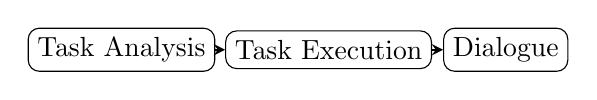
\begin{tikzpicture}
\node (task) [rectangle, rounded corners,text centered, draw=black,node distance=2.5cm] {Task Analysis};
\node (exec) [rectangle, rounded corners,text centered, draw=black, right of=task, node distance=2.63cm] {Task Execution};
\node (dial) [rectangle, rounded corners,text centered, draw=black, right of=exec,node distance=2.25cm] {Dialogue};
\tikzstyle{arrow} = [thick,->,>=stealth]
\draw [arrow] (task) -- (exec);
\draw [arrow] (exec) -- (dial);
\end{tikzpicture}
\caption{Recommendation Model}
\label{fig:rec-model}
\end{figure}

\paragraph{Characterizing peer interactions.} We explored five characteristics of peer interactions: Politeness, Persuasiveness, Receptiveness, Time Pressure, and Tool Observability. These characteristics were motivated from research in psychology and qualitative results from Murphy-Hill's prior work on peer interactions~\cite{Murphy-Hill2015HowDoUsers}. We used prior work in other fields to compile a list of criteria for these characteristics defined with examples from this evaluation in Table~\ref{tab:defs}. For each characteristic, we analyzed comments made in the dialogue between participants during peer interactions to observe these criteria. 

\textit{1) Politeness:} Research suggests politeness is important for making effective recommendations. For example, Whitworth suggests the reason Microsoft's Clippy recommender system was unsuccessful is because it was
impolite~\cite{WhitworthPolite}. 
Murphy-Hill and colleagues found that 
respect and trust 
were important factors in 
peer interactions for software engineers~\cite{Murphy-Hill2015HowDoUsers}. 
To measure politeness,
we used Leech's six maxims for politeness: 
Tact, Generosity, Approbation, Modesty, 
Agreement, and Sympathy~\cite{LeechPragmatics}.

\textit{2) Persuasiveness:} Prior work in persuasion theory suggests it is vital for making effective suggestions. For example, O'Keefe argues that in a wide variety of settings from courtrooms to families, ``human decision making is shaped by persuasive communication"~\cite[p.~31]{okeefe2002persuasion}. Fogg also suggests that persuasiveness is necessary to convince users to adopt desired behaviors through software~\cite{Fogg2009Persuasive}. Shen et al. present three features of persuasive messages that were used to measure persuasiveness in peer recommendations between participants in this study: Content, Structure, and Style~\cite{ShenMessageFeatures}.

\textit{3) Receptiveness:} Prior work shows that receptivity is important for making effective suggestions. For example, Fogg outlined best practices for creating
persuasive technologies to persuade users to adopt target behaviors. One key practice is to choose an ``audience that is most likely to be receptive to the targeted behavior" ~\cite{Fogg2009Persuasive}. Fogg provides two criteria to define a receptive audience: Demonstrate Desire and Familiarity. Users who demonstrate desire express interest in discovering, using, or learning more information about target behaviors while users with familiarity express knowledge about the target behavior or environment.

\textit{4) Time Pressure} Research suggests time pressure can impact the outcome of recommendations. For example, 
Andrews and Smith found that time constraints impact decision-making 
in marketing~\cite{AndrewsTimePressure}. 
Additionally, Murphy-Hill and colleague identified time pressure as a barrier to peer interactions in the form of project deadlines~\cite{Murphy-Hill2015HowDoUsers}. 
We did not strictly enforce a time limit for completing tasks in this study, but the suggested time was one hour. We measured time pressure by looking for statements 
mentioning time from participants and categorized peer interactions as either having time pressure or not.

%If we determined a statement was made regarding time, then we categorized the recommendation as being under time pressure. For example, during one study L13 was driving and noted ``I think we have like, four minutes left", ignoring L14's recommendation to use the \textsc{IF} function in Excel. Time pressure caused the driver to continue using her own methods and limited exploratory thinking for completing the task.

\textit{5) Tool Observability} Murphy-Hill and colleagues suggest that recommendations from 
systems should have noticeable causes and effects~\cite{Murphy-Hill2015HowDoUsers}. 
To analyze this, we examined the observability of tools recommended between participants in the study. Observability refers to whether or not tools are visible to users through a graphical user interface. To determine if the perception of tools impacts recommendations, we analyzed tools suggested between peers in our study and categorized them as Observable or Non-observable. 

\begin{table*}
\centering
\caption{Peer interaction characteristics from \peer study}
    \begin{tabular}{ |l|l|p{10cm}| }
	\hline
	\multicolumn{3}{ |c| }{\textbf{Politeness Criteria}} \\
	\hline
	\multirow{3}{*}{Tact} 
	 & Definition & Minimize cost and maximize benefit to peer \\
	 & Polite & ``We can do all of it together, just sort by level.'' - S9 \\
	 & Impolite & ``We can do a histogram...which is always sort of a pain in the butt to do in Excel.'' - L14 \\ \hline
	\multirow{3}{*}{Generosity} 
	 & Definition & Minimize benefit and maximize cost to self \\
	 & Polite & ``CONCATENATE you can do. I can do this for
you, very easily.'' - S10 \\
	 & Impolite & ``Maybe you should write a python script for this.'' - L6 \\ \hline
	\multirow{3}{*}{Approbation} 
	 & Definition & Minimize dispraise and maximize praise of peer \\
	 & Polite & ``I'm not as good at the Excel stuff as you are.'' - L5\\
	 & Impolite & ``This[partner's suggestion] is useless.'' - S14 \\ \hline
	\multirow{3}{*}{Modesty} 
	 & Definition & Minimize praise and maximize dispraise of self \\
	 & Polite & ``From whatever limited knowledge of data analysis I have, I think you need to create a linear regression model...'' - S14 \\
	 & Impolite & ``I'm very good at Paint.'' - S10 \\ \hline
	\multirow{3}{*}{Agreement} 
	 & Definition & Minimize disagreement and maximize agreement between peers \\
	 & Polite & ``Do you want to use Python?'' - S8 \\
	 & Impolite & ``No, no, no...Don't you want it comma separated? That's what I'm doing.'' - S14 \\ \hline
	\multirow{3}{*}{Sympathy} 
	 & Definition & Minimize antipathy and maximize sympathy between peers\\
	 & Polite & ``We can try JMP...'' [``I haven't done anything in JMP.''] ``Neither have I!'' - L14 \\
& Impolite & ``It doesn't matter how you do it.'' - L16 \\ \hline
    \hline
	\multicolumn{3}{ |c| }{\textbf{Persuasiveness Criteria}} \\
	\hline
	\multirow{3}{*}{Content} 
	 & Definition & Recommender provides credible sources to verify use of the tool\\
	 & Persuasive & ``Go here, go to Data. Highlight that...Data, Sort, and it lets you pick two.'' - L8 \\
	 & Unpersuasive & ``Let's try to text filter, right?'' - S5 \\ \hline
	\multirow{3}{*}{Structure} 
	 & Definition & Messages are organized by climax-anticlimax order of arguments and conclusion explicitness \\
	 & Persuasive & ``I know that SUMIF is a type of function that allows you to combine the capabilities of SUM
over a range with a condition that needs to be met.'' - S3\\
	 & Unpersuasive & ``There's a thing on Excel
where you can do that, where you can say if it is this value, include, if it is not, exclude...Yeah, IF.'' - S11 \\ \hline
	\multirow{3}{*}{Style} 
	 & Definition & Messages should avoid hedging, hesitating, questioning intonations, and powerless language \\
	 & Persuasive &  ``Click on title and do a Ctrl-A" - S13\\
& Unpersuasive & ``I guess we're going to have to use some math calculations here, or a pivot table.'' - L9 \\ \hline
    \hline
	\multicolumn{3}{ |c| }{\textbf{Receptiveness Criteria}} \\
	\hline
	\multirow{3}{*}{Demonstrate Desire} 
	 & Definition & Participant shows interest in using or learning more about a tool \\
	 & Receptive & ``That was cool, how [the column] just populated.'' - S4 \\
	 & Unreceptive & [``So you want to use R for it?''] ``No, no, no...'' - S14 \\ \hline
	\multirow{3}{*}{Familiarity} 
	 & Definition & Participant explicitly expresses familiarity with the environment \\
	 & Receptive & ``Control shift...how do I select it completely?'' - S2 \\
	 & Unreceptive & ``I've never done anything in JMP.'' - L10 \\ \hline
	\hline
	\multicolumn{3}{ |c| }{\textbf{Time Pressure Criteria}} \\
	\hline
	\multirow{3}{*}{Time Pressure} 
	 & Definition & Participant makes statement regarding time to complete tasks \\
	 & Yes & [Python script] ``Yeah, that would work, if we had time.'' - L5 \\
	 & No & No comments about time \\ \hline
	\hline
	\multicolumn{3}{ |c| }{\textbf{Tool Observability Criteria}} \\
	\hline
	\multirow{3}{*}{Observability} 
	 & Definition & The ability to view a tool through a GUI \\
	 & Observable & ``Let's deploy a histogram...Insert, Recommended Charts...'' - S7 \\
	 & Non-Observable &  ``Control-Shift-End'' - S1 \\ \hline
\end{tabular}
\label{tab:defs}
\end{table*}

\paragraph{Determining the effectiveness of peer interactions.} To measure effectiveness, each software tool recommendation between participants was categorized as \textit{effective}, \textit{ineffective}, and \textit{unknown}. For effective recommendations, the recommendee used a tool after it was suggested by their partner for the remainder of their session for a majority of the opportunities it was applicable. For ineffective recommendations, the recommendee mostly ignored a tool recommended by their partner when they had a chance to utilize it in the study. Finally, unknown recommendations were the case where there was not another opportunity for the recommendee to use a suggested tool for the rest of their study session. Two researchers independently viewed recordings of each session to note instances of tool recommendations and categorize the peer interactions based on the criteria defined for politeness (Cohen's $\kappa$ = 0.50), persuasiveness (Cohen's $\kappa$ = 0.28), and 
receptiveness (Cohen's $\kappa$ = 0.51). The coders came together to discuss and resolve any disagreements.

\begin{table*}[!htbp]
\centering
\caption{\peer Study Results}
\resizebox{.7\textwidth}{!}{%
\begin{tabular}{|l|lll|lll|lll|}
\hline
  \multirow{2}{*}{}  &  \multicolumn{3}{c|}{Effective} & \multicolumn{3}{c|}{Ineffective} & \multicolumn{3}{c|}{Unknown}  \\
\cline{2-10}
 & \textit{n} & & \% & \textit{n} & & \% & \textit{n} & & \% \\
\hline
\multicolumn{8}{|l}{\textit{Politeness}} &  & \\
\hline
Polite & 14 & \posbar{.52} & 52\% & 5 & \posbar{.19} & 19\% & 8 & \posbar{.30} & 30\% \\
Neutral & 52 & \neutralbar{.5} & 50\% & 27 & \neutralbar{.26} & 26\% & 25 & \neutralbar{.24} & 24\% \\
Impolite & 5 & \negbar{.45} & 45\% & 3 & \negbar{.27} & 27\% & 3 & \negbar{.27} & 27\%\\
\hline
\multicolumn{8}{|l}{\textit{Persuasiveness}} &  & \\
\hline
Persuasive & 5 & \posbar{.36} & 36\% & 4 & \posbar{.29} & 29\% & 5 & \posbar{.36} & 36\% \\
Unpersuasive & 66 & \negbar{.52} & 52\% & 31 & \negbar{.24} & 24\% & 31 & \negbar{.24} & 24\%\\
\hline
\multicolumn{8}{|l}{\textit{Receptiveness*}} &  & \\
\hline
Receptive & 39 & \posbar{.61} & 61\% & 9 & \posbar{.14} & 14\% & 16 & \posbar{.25} & 25\% \\
Neutral & 27 & \neutralbar{.48} & 48\% & 14 & \neutralbar{.25} & 25\% & 15 & \neutralbar{.27} & 27\% \\
Unreceptive & 5 & \negbar{.23} & 23\% & 12 & \negbar{.55} & 55\% & 5 & \negbar{.23} & 23\%\\
\hline
\multicolumn{8}{|l}{\textit{Time Pressure}} &  & \\
\hline
Yes & 7 & \posbar{.37} & 37\% & 7 & \posbar{.37} & 37\% & 5 & \posbar{.26} & 26\% \\
No & 64 & \negbar{.52} & 52\% & 28 & \negbar{.23} & 23\% & 31 & \negbar{.25} & 25\%\\
\hline
\multicolumn{8}{|l}{\textit{Tool Observability}} &  & \\
\hline
Observable & 57 & \posbar{.50} & 50\% & 30 & \posbar{.26} & 26\% & 28 & \posbar{.24} & 24\% \\
Non-Observable & 14 & \negbar{.52} & 52\% & 5 & \negbar{.19} & 19\% & 8 & \negbar{.30} & 30\% \\
\hline
\multicolumn{8}{|l}{\textit{Recommendation Type}} &  & \\
\hline
Peer Observation & 16 & \posbar{.30} & 30\% & 5 & \posbar{.09} & 9\% & 32 & \posbar{.60} & 60\% \\
Peer Recommendation & 55 & \negbar{.62} & 62\% & 30 & \negbar{.34} & 34\% & 4 & \negbar{.05} & 5\%\\
\hline
\end{tabular}%
}
\label{tab:interactions_effect}
\end{table*}

\subsubsection{Results:}

In total, we discovered 142 total recommendations between participants in out study: 71 effective; 35 ineffective; and 36 unknown. Table~\ref{tab:interactions_effect} presents the breakdown of effectiveness for each characteristic we examined in our study. Out of the peer interaction characteristics we analyzed, \textit{receptiveness} was the only characteristic that significantly impacted the outcome of a tool recommendation between peers (Wilcoxon, \textit{p} = 0.0002, $\alpha$ = .05). These results indicate that the receptiveness of users is what makes recommendations to developers effective. In this study, we defined receptiveness using two criteria from prior work by Fogg on designing persuasive technology: \textit{\textbf{Demonstrate Desire}} and \textit{\textbf{Familiarity}}~\cite{Fogg2009Persuasive}. We suggest integrating these concepts into automated recommendations for developer actions to software engineers to improve the effectiveness of suggestions and increase adoption of useful programming tools and practices. These results were published in the 2017 Visual Languages and Human-Centric Computing (VL/HCC) conference~\cite{VLHCC}.


\subsection{[\sorryT] ``Sorry to Bother You: Designing Bots for
Effective Recommendations" (Completed, Spring 2019)}

\subsubsection{Motivation:}

While recommendations between humans are the most effective, they are not always the most practical way to increase awareness of useful development tools. For example, even though Murphy-Hill and colleagues discovered that developers prefer peer interactions for tool discovery, they also found that peer interactions occur less frequently in the workplace~\cite{Murphy-Hill2011PeerInteraction}. As development teams become larger and more distributed, effective automated recommendations are necessary to improve tool adoption among software engineers. Research shows bots are useful for automating tasks and improving user effectiveness and efficiency~\cite{StoreyBots}. However, they can also be inconvenient and frustrating during interactions with humans. To better understand the impact of bots and identify a baseline for automated recommendations, we created \tool to make development tool recommendations to software engineers on GitHub using a \tele. In this study, we examined the effectiveness of recommendations from \tool and gathered feedback from developers who received a suggestion to better understand user reactions to receiving naive automated recommendations and set the groundwork for designing better solutions in future approaches.


\subsubsection{\tele:}

To evaluate a basic design for making automated recommendations, we developed \tele. This approach behaves similar to a telemarketer in that it ``calls" users to deliver a static message that never deviates from the script and lacks the social context necessary to adjust messages, customize recommendations, or respond to questions and feedback. \tele sends developers a generic message with information about a static analysis tool, displays a generic example featuring a code snippet based on a common programming error, and provides sample output from the tool. This is not the best approach for making recommendations, however we implemented this simple design to better understand how bots influence human behavior and how developers respond to automated recommendations. With this naive design, we developed a simple bot to evaluate and identify a baseline for making automated recommendations for developers. We use our results and feedback from developers to motivate integrating concepts from nudge theory to improve future automated recommendation designs. 

\subsubsection{Methodology:}

\paragraph{Data Collection.}

Our evaluation sought to determine the effectiveness of our \tele recommendation approach to developers working on real-world software applications. We randomly sampled public open source software repositories on GitHub used in the evaluation for Repairnator\footnote{\url{https://github.com/Spirals-Team/repairnator/blob/master/resources/data/results-buildtool.csv}}~\cite{Repairnator}, an automated program repair bot~\cite{Repairnator}. The projects selected for this study had to meet the following criteria:

\begin{itemize}
    \item written in Java 8 or higher,
    \item successfully validate and compile with Maven,
    \item do not already include \EP in the build configuration
\end{itemize}

Based on these criteria, we identified 52 projects for our experiment that received an automated pull request recommendation. The list of projects for this evaluation is available online\footnote{\url{https://go.ncsu.edu/botse-projects}}.

\paragraph{Implementing the \tele.} To evaluate our \tele approach, we implemented \tool to make basic tool recommendations to GitHub developers. \tool integrates this simple approach by making generic recommendations as automated pull requests on repositories. On GitHub, pull requests are the preferred method to propose changes to repositories\footnote{\url{https://help.github.com/articles/about-pull-requests/}}. Automated pull requests have also been used by bots in related work, for example by Mirhosseini and colleagues to encourage GitHub developers to upgrade out-of-date dependencies for repositories~\cite{SamUgrade}. Figure~\ref{fig:tele} presents a screenshot of a recommendation from our system for this study. In this experiment, \tool recommendations provided basic information about the Java static analysis tool \EP  (Fig.~\ref{fig:tele}.A). It also presents a simple coding error in Java, using ``\texttt{==}" to evaluate string equality instead of the \texttt{String.equals()} method (Fig.~\ref{fig:tele}.B1), and the corresponding output from \EP reporting a \texttt{StringEquality} error\footnote{\url{http://errorprone.info/bugpattern/StringEquality}} (Fig.~\ref{fig:tele}.B2). To make recommendations, \tool automatically adds the \EP plugin to Maven\footnote{\url{http://maven.apache.org}}, to Project Object Model (\textit{pom.xml}) configuration files and created automated pull requests with the changes. An example pull request from our system using the \tele can be found here.\footnote{\url{https://github.com/CSC-326/JSPDemo/pull/2}}

\begin{figure}
\centering
	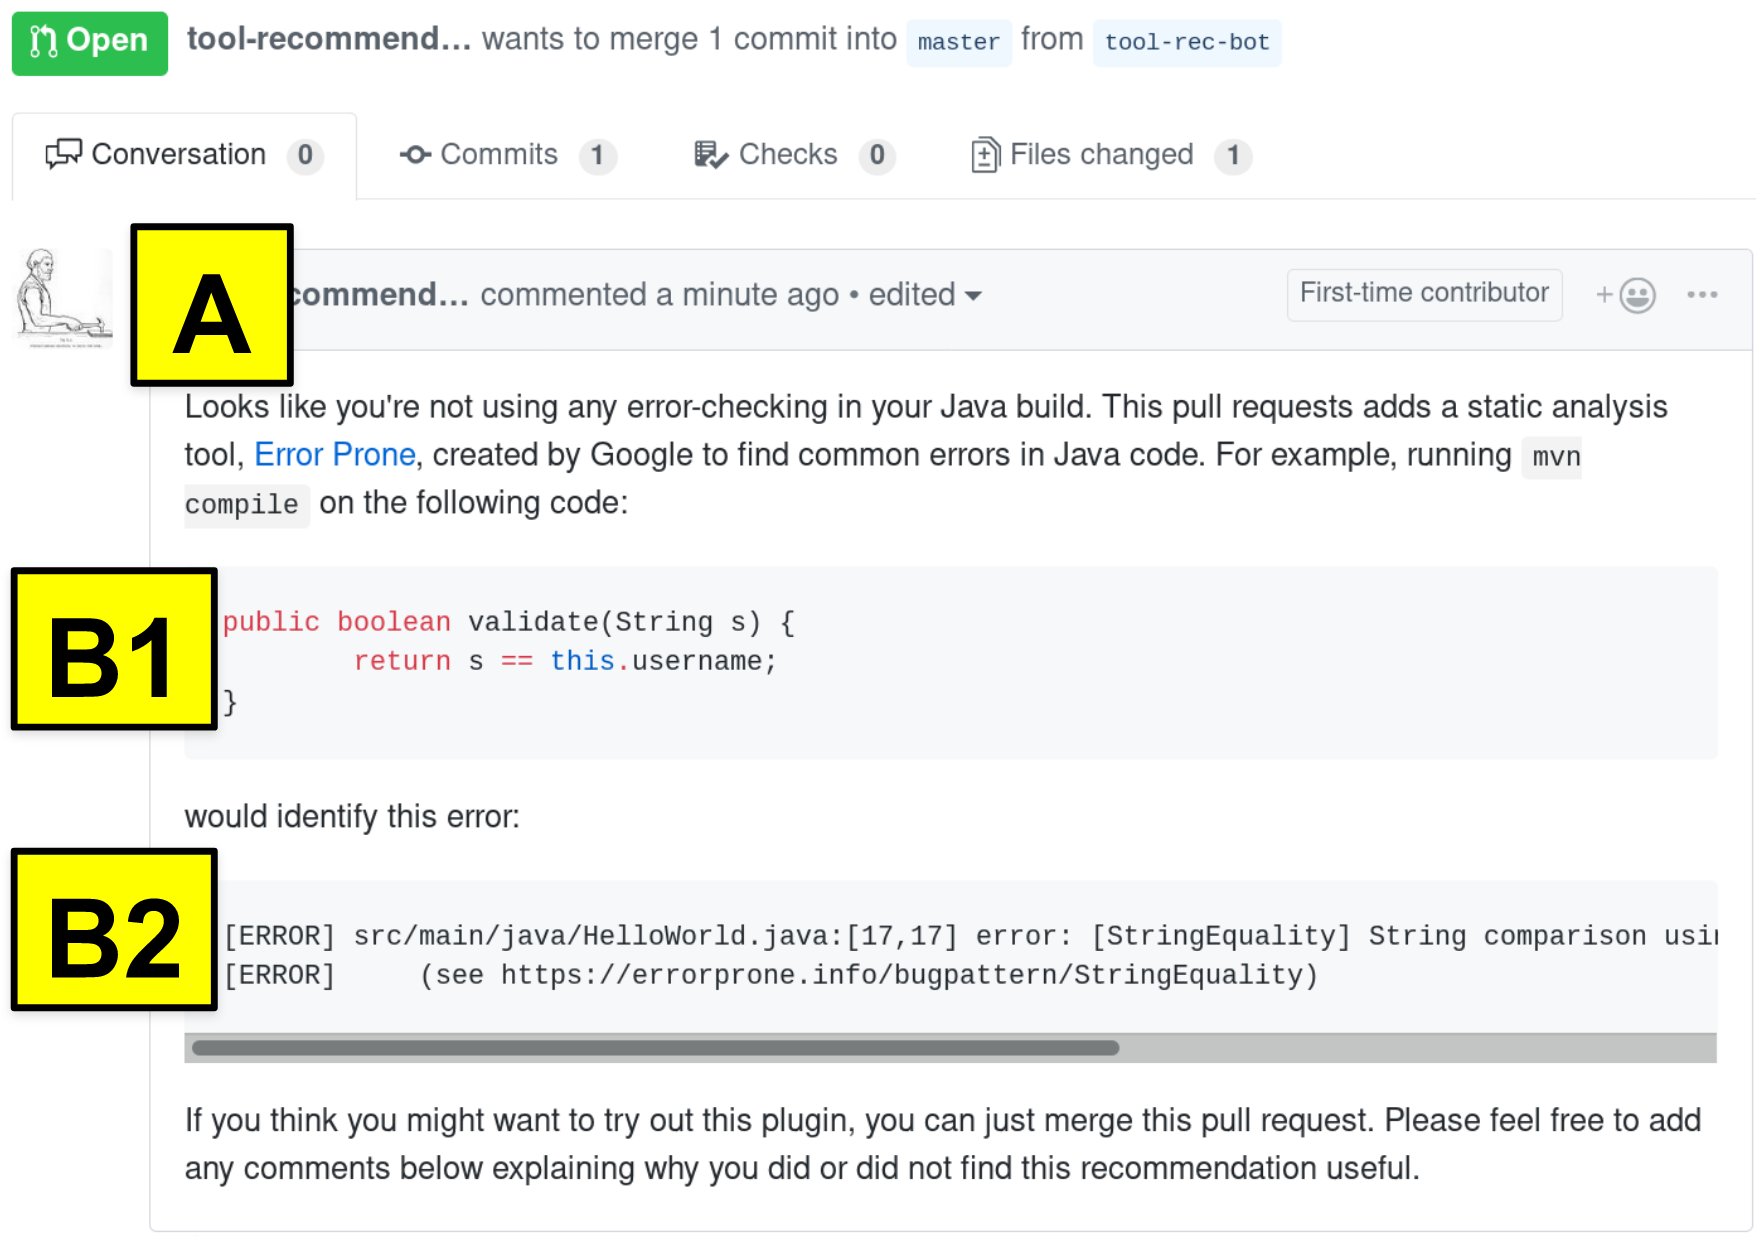
\includegraphics[width=0.5\textwidth]{images/pull.png}
	\caption{Example \tele recommendation}	
	\label{fig:tele} 
\end{figure}

\paragraph{Determining the effectiveness of recommendations.}

To measure the effectiveness of \tele, we observed the status of automated pull requests from \tool. A merged automated pull request from \tool indicates an effective recommendation because the developer showed a willingness to try \EP and integrate the static analysis tool  into the build for their repository by merging our changes into their code base. A closed or ignored pull request left open from our system indicates an ineffective recommendation because the developers did not attempt to integrate the tool into their projects. We observed the automated pull requests for one week to categorize the recommendations. The rate of effectiveness was calculated by measuring the percentage of merged pull requests out of the total sent.

Additionally, we encouraged developers to provide feedback on pull requests by asking them to ``Please feel free to add any comments below explaining why you did or did not find this recommendation useful". This was done to gather qualitative data on how developers reacted to receiving \tele recommendations from \tool. We aggregated and analyzed the comments made by GitHub developers on our automated recommendations. Figure~\ref{fig:botse} presents a screenshot of example automated pull requests used in the evaluation for this study.

\begin{figure*}[]
\centering
\subfloat[Pull request recommendation text]{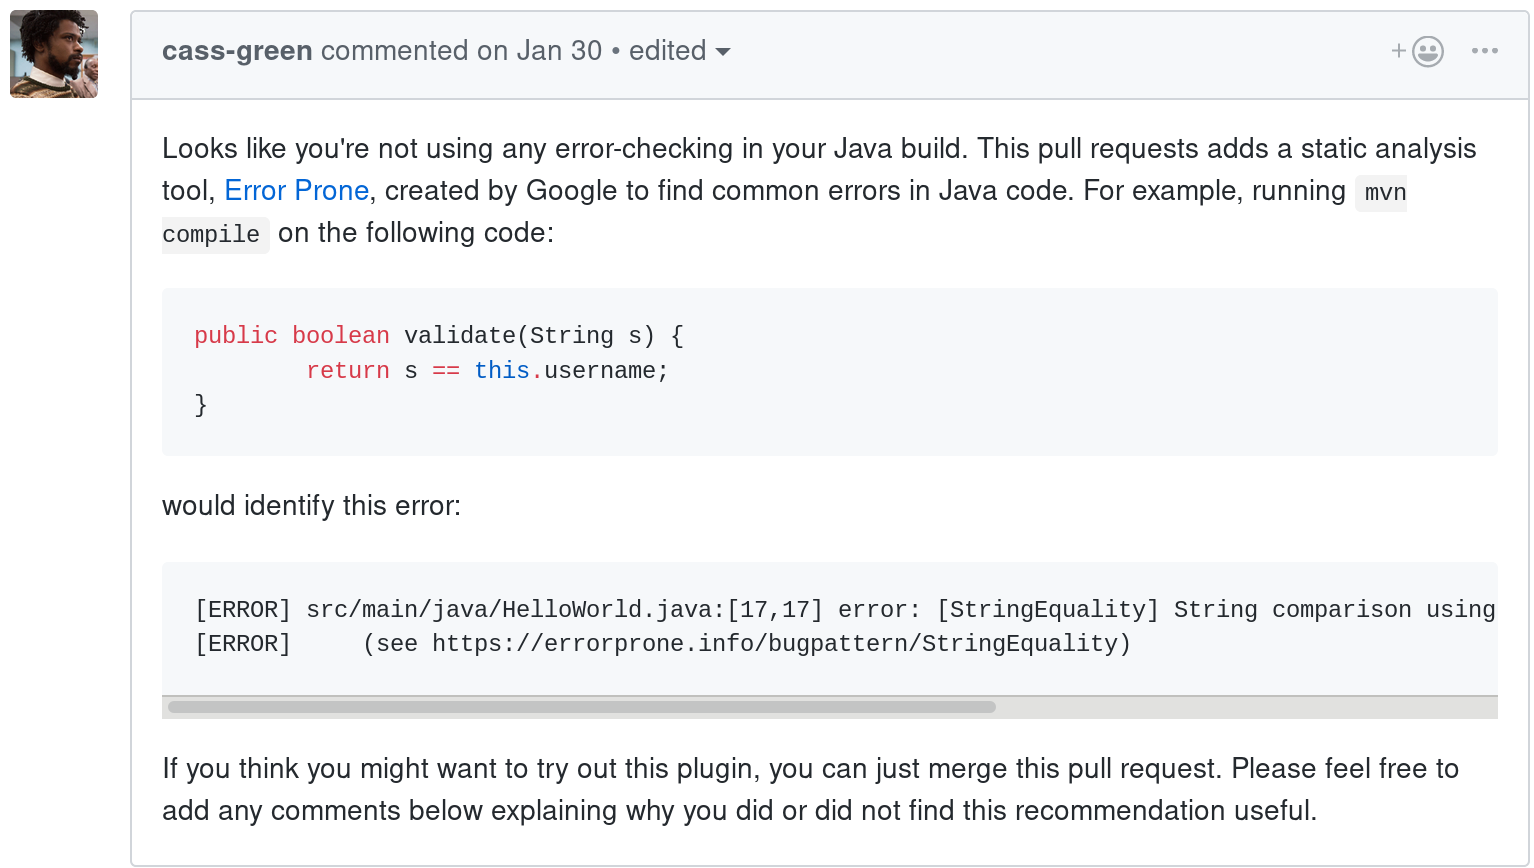
\includegraphics[width=0.5\linewidth]{images/botse1.png}}
\subfloat[Pull request diff updating a \pom file]{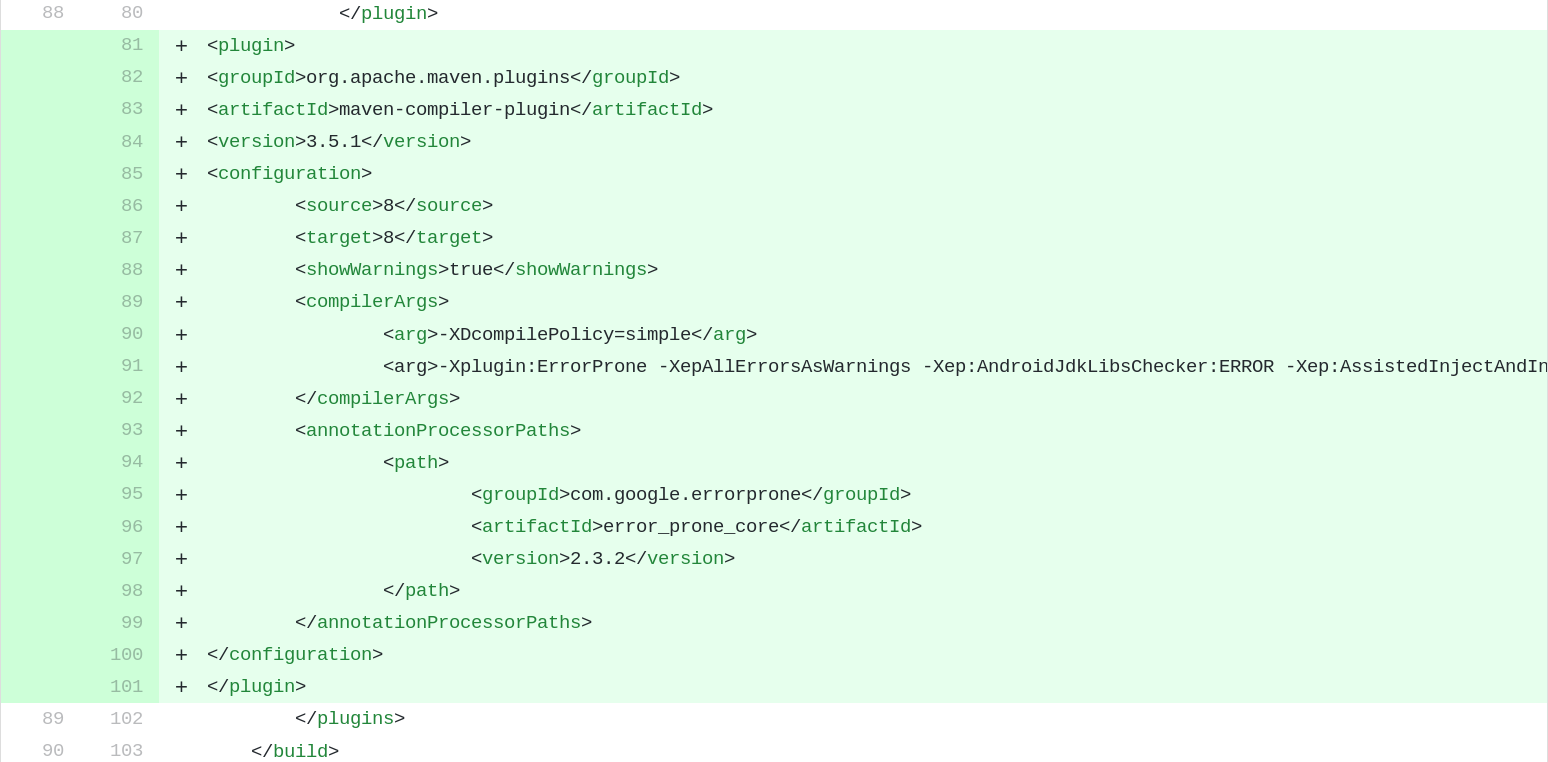
\includegraphics[width=0.6\linewidth]{images/botse2.png}}
\caption{Example automated pull request from the \sorry study}
\label{fig:botse}
\end{figure*}

\subsubsection{Results:} 

We found that bots with basic approaches are not effective for influencing human behavior. Table~\ref{tab:sorry_results} presents our findings from the evaluation. In our study, \tele only made two successful recommendations out of 52 (4\%). We also observed 10 closed pull requests and 40 recommendations with no response from developers. We received 18 comment responses from developers, most of which were negative feedback. Five of the comments were related to improper formatting of the \textit{pom.xml} file when adding the \EP plugin, and eight were related to our automated pull requests breaking builds for projects. Based on this feedback, we discovered the main drawbacks to the \tele were a lack of \textit{\textbf{social context}} and interfering with \textit{\textbf{developer workflow}}. To provide implications for future automated recommender systems, we propose integrating concepts from nudge theory to effectively incorporate automated suggestions for developer actions in software engineers' social context and development workflow. The results of this research were published and presented at the 1st International Workshop on Bots in Software Engineering\footnote{\url{https://botse.github.io/}} (BotSE 2019) at the International Conference on Software Engineering (ICSE)~\cite{BotSE}.

\begin{table}[H]
\centering
\begin{tabular}{ |c|c|c| } \hline
  & \textit{\textbf{n}} & \textbf{Percent} \\ \hline
 Merged & 2 & 4\% \\ \hline 
 Closed & 10 & 19\% \\ \hline
 No Response & 40 & 77\%\\ \hline 
\end{tabular}
\caption{\sorry Study Results}
\label{tab:sorry_results}
\end{table}


\section{Developer Recommendation Preconditions}

Based on the results from these preliminary studies, we uncovered four concepts for making effective developer recommendations. At the minimum, these developer recommendation preconditions are required to make successful recommendations for software engineers. Below we define each of these concepts and provide examples with data collected from the completed evaluations, other software engineering research, and nudge theory literature:

\subsection{Demonstrate Desire}

In the \peer~study, we found that participants expressing  eagerness  to  use  a  recommended  tool led to more effective recommendations.  For example, during one study session a participant suggested using multi-level sorting functionality in Excel. Their partner, L11, demonstrated a desire to use the tool by  responding ``Oh!  Add  level!  Yes, awesome!" and adopted multi-level sorting for the remainder of the study tasks. This suggests recommending desirable tools and behaviors can increase adoption among developers. Meanwhile, in another case a participant asked their partner if they wanted to use the R statistical computing software\footnote{\url{https://www.r-project.org/}} to complete a task, but their partner responds ``No, no, no..." (S14). This shows how a lack of desire to use a specific tool can negatively impact the outcome of a recommendation. 

Software engineering research also suggests desire impacts the activities and behavior of developers. For example, Senyard and colleagues suggest that the desire of developers is important for motivating programmers to contribute to free and open source software and maintain successful projects~\cite{senyard2004have}. Furthermore, Murphy-Hill and colleagues found that one barrier to peer interactions is \textit{developer inertia}. This refers to when programmers do \textit{not} desire to share or learn about new software engineering tools because they ``feel that they do not need to discover a new tool because existing tools will do the job"~\cite[p.~16]{Murphy-Hill2015HowDoUsers}. These are examples of how the desire of software engineers can impact their behavior and decision-making when completing programming tasks.

Behavioral science research shows that humans often make poor decisions based on their desires. This is due to the fact that sometimes damaging behaviors provide short term benefits but have long term costs. Examples of these activities include smoking and eating junk food. Sunstein and Thaler argue humans need decision-making help in situations when ``choices and their consequences are separated in time...we get the pleasure now and suffer the consequences later...[these] are prime candidates for nudges"~\cite[p.~75]{sunstein2008nudge}. Nudges can be used to encourage the adoption of better behaviors by raising awareness of consequences for decisions. For example, nudges to teenagers in Montana were able decrease smoking rates among students by educating them on the dangers of smoking and providing information on the behaviors of peers~\cite{linkenbach2003most}. In some cases, poor developer behaviors may provide benefits to development teams. For example, Xiao and colleagues found that developers avoid adopting security tools that automatically check for vulnerabilities in code to save time and costs for training and implementing new systems~\cite{Xiao2014Security}. While avoiding useful developer behaviors may provide some benefits such as saving time and money, ignoring these practices can ultimately have serious consequences for development teams and their products over time. Nudges such as providing improved and more relevant feedback to users are an effective way to persuade developers to adopt better behaviors they may find undesirable by providing information and insight into the long term costs of avoiding these actions. 

\subsection{Familiarity}

Another key takeaway from the \peer~study is that users are more likely to adopt recommendations for tools and concepts they are familiar with it. In this study, we defined this criteria as users explicitly expressing familiarity with the environment surrounding a recommended tool. An example of an familiarity impacting the outcome of a recommendation in our experiment arose when L8 asked about using the \texttt{COUNTIF} function in Excel. L7 was familiar with the function and used the tool replying ``Yeah...here we go". However, we also found unfamiliarity negatively influenced adoption when a participant recommended using R to create a plot for analyzing the data, but their partner responded ``I don’t know R" (S9). In this case, the participant's unfamiliarity with R led to an ineffective recommendation. 

Familiarity can also lead to \textit{developer inertia}, where programmers prefer to stick with their familiar tools and workflow and avoid adopting better behaviors. Prior research also suggests familiarity can impact effectiveness and productivity at work. Goodman and colleagues found that the more knowledge employees have about the workplace and environment, or \textit{work familiarity}, improves performance~\cite{goodman1992familiarity}. Similarly in software engineering, Espinosa and colleagues found that familiarity impacts the completion of development tasks for distributed development teams~\cite{espinosa2002shared} while de Alwis and colleagues found that unfamiliarity in the Eclipse IDE made developers feel disoriented and negatively impacted productivity~\cite{de2006using}. For improving development tool adoption, Murphy-Hill and colleagues propose integrating familiarity into recommender systems by ranking commands based on similarity with collaborative filtering~\cite{Murphy-Hill2012Fluency}. Finally, Ko and colleagues suggest the majority of developers' time is spent learning about and becoming familiar with unfamiliar code, and code comprehension can impact other development activities and behaviors such as code navigation, searching, and tool usage~\cite{ko2006exploratory}. This indicates that familiarity plays a role in developer behavior and impacts their adoption of useful practices.

Research suggests humans are prone to make decisions based on previous experiences and rarely select options that are unfamiliar. Thaler and Sunstein note ``it is particularly hard for people to make good decisions when they have trouble translating the choices they face into the experiences they will have...when people have a hard time predicting how their choices will end up affecting their lives...a nudge might be welcomed"~\cite[p.~77-78]{sunstein2008nudge}. One example of an unfamiliar problem for many families face is selecting student loans. To account for unfamiliarity in student loan selections, Bettinger and colleagues implemented a nudge to incorporate the Free Application for Federal Student Aid (FAFSA) for student financial aid into the H\&R Block\footnote{\url{https://www.hrblock.com}} tax return software, which many are more familiar with and utilize annually to complete their taxes. They found that this nudge made it easier to compare loan options and increased college enrollment among high school seniors~\cite{bettinger2013fafsa}. Many software engineers are comfortable with their current toolsets and environments, which leads to an unwillingness to try new useful development tools and processes. Nudges such as providing more information to software engineers when recommending unfamiliar development tools can help increase awareness and inform developers of new and better systems for completing programming tasks over their familiar methods.


\subsection{Social Context}

In the results from the \sorry~study, we found that one major issue with our \tele design is its lack of social context. Social context refers to the standard practices and activities necessary to participate in software engineering by interacting with developers and contributing to projects, specifically in open source software. In the \sorry~evaluation, many developers complained that \tool did not adhere to formatting guidelines when automatically adding the \EP plugin to project \textit{pom.xml} files. The most common social context complaint we received from GitHub users was that \tool messed up the whitespace of their project's maven \pom files when adding the \EP plugin (See Figure~\ref{fig:botse}b). One developer replied ``The automated tool you use messed up the pom.xml formatting to an extent that I could not see it" (P5). This suggests our bot's inability to adjust to the social context surrounding software development negatively impacted developers' likelihood to adopt recommendations.

Prior work also shows that social context is important in making recommendations to software engineers. Ahmadi goes as far as to argue that software engineering is a social activity~\cite{ahmadi2008survey}. To make effective recommendations, studies show it is important to integrate into this social context. For example, Wessel and colleagues evaluated the usage of bots in open source software and found that their inability to integrate into contributors' social context due to limited decision-making and poor feedback was the biggest challenge developers face interacting with bots and desired better interactions with users~\cite{wessel2018power}. Furthermore, prior work found that bots emulating humans receive better responses from developers and are more effective than recognizable bot accounts~\cite{murgia2016among}. Thus, effectively integrating recommendations with the social context of software engineering can impact developer adoption and perception of tools.

In \textit{Nudge}, the authors note ``one of the most effective ways to nudge (for good or evil) is via social influence"~\cite[p.~54]{sunstein2008nudge}. To study the impact of social nudges, Schultz and colleagues conducted a study that provided feedback to homeowners about the energy usage rates for their neighbors and households in a neighborhood in San Marcos, CA. They found that this nudge was able to drastically decrease usage and improve consumption decisions among users~\cite{schultz2007constructive}. Social recommendations are popular within software engineering. For example, badges are an effective way to present information about the status and condition of public projects, which can impact the behavior of contributors and other users~\cite{trockman2018badges}. In turn, we suggest nudges are an effective method to integrate recommendations for software engineers to adopt useful developer behaviors into the social environment of software engineering.

\subsection{Developer Workflow}

Another key result from \sorry was that the \tele in \tool disrupted the workflow of developers, or the processes required to complete programming tasks and deliver software. The most notable example of this was the fact that our automated pull requests for \EP often broke builds for repositories. Many projects have adopted continuous integration systems, such as TravisCI,\footnote{\url{https://travis-ci.org/}} to automatically build and integrate changes into projects. However, modifying projects to add a new static analysis tool often introduced many new errors and caused the build to fail. An example of this from our evaluation can be seen in Figure~\ref{fig:error}. Out of the 52 pull requests made, at least 17 resulted in a broken build. Many developers complained about this in their feedback on \tool, including P18 who commented ``This PR failed automatic checks, I think it should be closed". This interruption of developer workflow often discouraged users from merging pull requests from our system and accepting the recommendation.

Other work in software engineering also notes the importance of integration into the workflow of developers. For example, Sadowski found that one of the primary reasons developers at Google ignore static analysis tool warnings is because they are not integrated into their workflow~\cite{sadowski2018lessons}. Additionally, Viriyakattiyaporn and colleagues found that the inability to deliver suggestions within appropriate workflows discouraged programmers from following recommendations to improve code navigation with Spyglass~\cite{viriyakattiyaporn2009challenges} while Johnson and colleagues discovered that software engineers reported avoiding static analysis tools in their work due to a lack of customizability and poor integration into their existing processes~\cite{Johnson2013Why}. This points to a need to integrate recommendations to developer within their workflow to increase the adoption of useful behaviors to improve code quality and developer productivity. 

Nudges are useful for integrating recommendations into user workflows. For instance, a study conducted on Yale seniors found that a lecture on the risks of tetanus was ineffective (3\%) in convincing students to get a shot at the health center. However, providing a campus map to students with the health center circled in the same lecture convinced over nine times more people (28\%) to get the shot~\cite{leventhal1965specificity}. Even though the first group of students knew the location of the health center, nudges such as providing more details allowed students to know how to fit a visit into their weekly schedule and normal workflow. Software engineering research shows that integration into developer workflows is vital. To improve on the lack of tool adoption at Google, Sadowski implemented Tricorder to run numerous program analysis tools on code during code reviews~\cite{Tricorder}. Similarly, Balachandran found that integrating tools into the code review process with Review Bot at VMWare was able to reduce developer effort and improved code quality during code inspections~\cite{balachandran2013reducing}. These studies provide examples of how integration into developer workflow increased adoption of development tools. We believe this concept is key to improving the effectiveness of developer recommendations and encouraging adoption of useful developer behaviors.





% High spatial locality

% %\subsection{\timing}

% Location (hot and cold) [nudge theory] finds that timely feedback can improve acceptance of suggestion. Examples of these in real life? For example, handing out floss, right before entering a bathroom after eating ribs, increased chances of adopting flossing by 20\% (\todo{replace with example not completely made up}).

% To evaluate the timing of digital nudges, we introduce the concept of \emph{just-in-time nudges}. These nudges make recommendations to developers at a moment when a software engineering behavior is appropriate.

% We hypothesize that developers will prefer just-in-time nudges when a software engineering tool is most applicable over nudges presented at different times. Recommendations made when they are appropriate provide more convenience to users so developers don't have to figure out when's the best time to use a tool or practice. This can help improve adoption of software engineering behaviors for developers while they are completing programming tasks. A potential downside to just-in-time nudges is that they can interrupt developers in their work, which research suggests may lead to a loss of task context~\cite{parnin2010interrupted}.

% High temporal locality

\begin{figure*}
\centering
	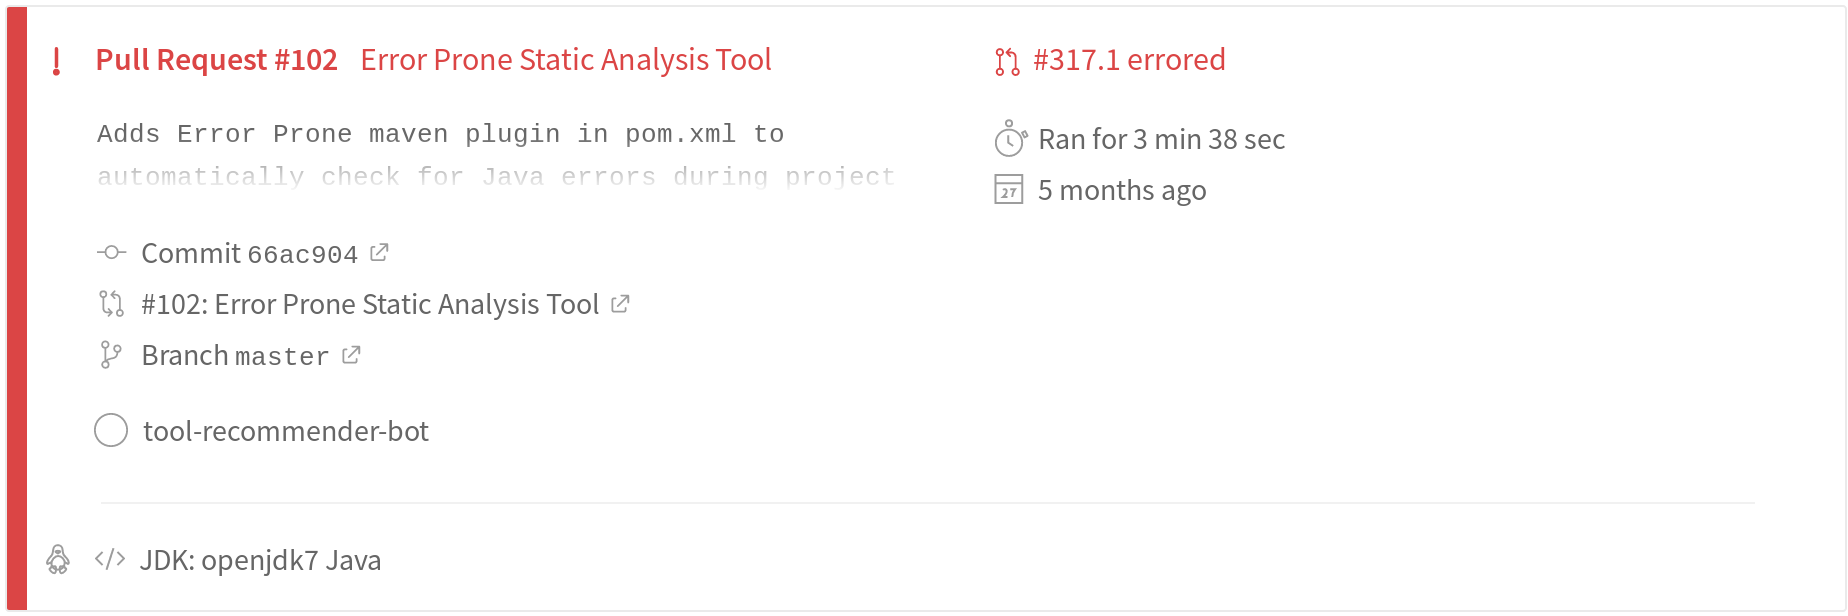
\includegraphics[width=\textwidth]{images/error.png}
	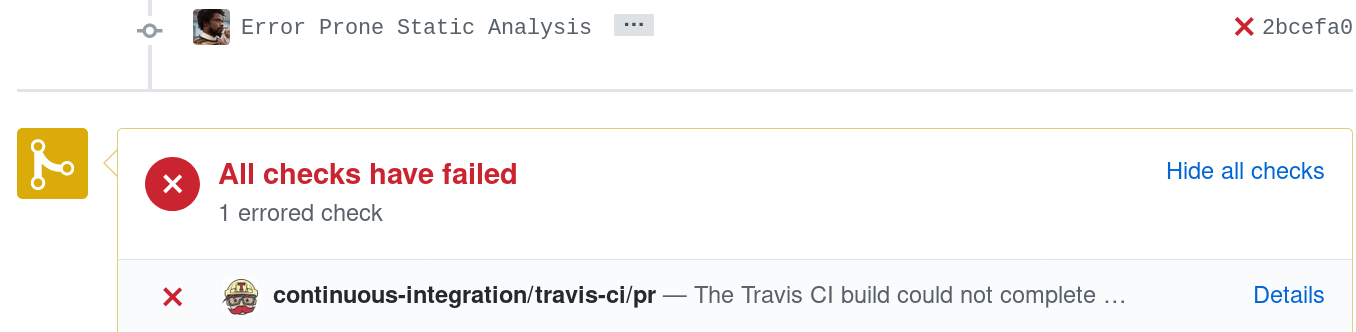
\includegraphics[width=\textwidth]{images/error2.png}
	\caption{Examples of automated pull requests from \tool causing projects' continuous integration builds to fail}	
	\label{fig:error} 
\end{figure*}


% %\subsection{Public nudge}

% %Humans are more likely to adopt behavior if there is external pressure to do so.

% %We define \textit{public nudges} as nudges that are visible and available to see by a specific community. They may also involve social pressure if certain behaviors aren't adopted. For example, badges on GitHub are public nudges viewable to users who visit a repository and can influence their decision to contribute or use the product. These badges display whether projects adopt certain software engineering behaviors, such as passing builds. Figure \ref{fig:red_badge} presents a badge for a project that does not use a useful software engineering processes during development, while the developers for a project with a badge in Figure \ref{fig:green_badge} integrate software engineering behaviors in their development process. Trockman and colleagues examined the effect of these public nudges for npm\footnote{https://www.npmjs.com/} packages on GitHub and found that the addition of badges correlated with improvements in the quality of the project, i.e. adding a quality assurance badge displaying code coverage increased the coverage of tests~\cite{trockman2018badges}

% %Our hypothesis is that developers are more likely to adopt useful software engineering behaviors if they are publicly nudged to do so.

% % \begin{figure}
% % \centering
% % \subfigure[Project without a software engineering behavior]{
% % \label{fig:red_badge}
% % 
\includegraphics[width=\textwidth/2]{images/badge1.png}}
% % \qquad
% % \subfigure[Project with a software engineering behavior]{
% % \label{fig:green_badge}
% % 
\includegraphics[width=\textwidth/2]{images/badge2.png}}
% % \caption{Example of a public nudge}
% % \end{figure}

% % [benefits/trade-offs;hypothesis]

% % \subsection{Social nudge}

% % Nudge theory finds that people are more likely to adopt a useful behavior if others they know already do it. Perloff studied the impact of social media on body image and self-perception among American girls, and proposes using ``media-based interventions...to nudge individuals into changing their attitudes and behaviors"~\cite[p.~364]{perloff2014social}. This work suggests social media use is key in creating social comparisons and influencing users to adopt harmful behaviors such as body dissatisfaction and eating disorders.

% % To study digital nudges in a social context, we introduce \textit{social nudges}. These nudges suggest software engineering behaviors that have been adopted by a developer's friends or colleagues. An example of this is seen in prior work examining peer interactions. Murphy-Hill conducted interviews and surveys with software engineers and found that developers prefer recommendations from peers over other methods of tool discovery such as tutorials, discussion threads, tool encounters, and written descriptions~\cite{Murphy-Hill2015HowDoUsers}.

% % Our hypothesis is that developers are more likely to adopt behaviors recommended in a nudge if they know it is used by a friend or colleague.

% % \subsection{Apprehensive nudge}

% % If you can show a target behaviors usefulness by presenting multiple places it can be applied, people are more likely to adopt it.

% % We created the concept of \textit{apprehensive nudges}, which provide multiple locations where software engineering activities can be applied, to study how this impacts activity adoption for developers.


% % \subsection{Automated nudge}

% % If you do the work for them, humans are more likely to adopt specific behaviors. \todo{Example= automatic magazine subscription renewal due to status quo bias [Nudge, 35]}

% % To determine if automatically performing software engineering behaviors for developers impacts adoption for developers, we introduce \textit{automated nudges}. There are many ways automation is used to improve software engineering and help developers adopt helpful behaviors. For instance, Mirhosseini and colleagues investigated creating automated pull requests to convince developers to upgrade outdated dependencies using greenkeeper\footnote{https://greenkeeper.io} to manage dependency package versions for GitHub projects~\cite{sam2017autopullrequests}. They found that automated pull requests were useful in increasing awareness of out-of-date package dependencies to developers.

% % [benefits/trade-offs;hypothesis]

% % \subsection{Tutorial nudge}

% % If you show people how to do a certain behavior, then they are more likely to adopt it.

% % We define \textit{tutorial nudges} as digital nudges that show developers how to use a specific software engineering tool or programming activity. For example,...

% % [Conceptual implementation]

% % [benefits/trade-offs;hypothesis]

% % \subsection{Reminder nudge}

% % If you continually remind humans to adopt a certain activity, they are more likely to adopt it.

% % To evaluate the effectiveness of reminders, we developed \textit{reminder nudges} to periodically recommend useful software engineering behaviors to programmers.

% % [Conceptual implementation]

% % [benefits/trade-offs;hypothesis]

% % \subsection{Positive nudge}

% % Nudge theory suggests using positive language is more effective in helping people adopt target behaviors. For example, Doberstein and colleagues evaluated using positive messages to improve attitudes about increasing residential housing density in Canada~\cite{doberstein2016positive}. They compared a neutral control statement of benefits with public statements, private statements, and expert comparisons.  \todo{Framing [Nudge, 36-37]}

% % To determine if developers respond better to positive or negative recommendations, we introduce \textit{positive nudges} that commend developers for their work rather than blaming them to encourage future software engineering behavior adoption.

% % \subsection{Effects}

% % We hope our nudges have some of the following effects on developers who receive recommendations for software engineering behaviors...

% % \todo{Some interesting effects to consider:}
% % \begin{itemize}
% % \item Baader-Meinhof --- you start seeing something you just learned or on your mind everywhere.
% % \item Diderot Effect --- the act of getting one new thing triggers a cascade of other new things.
% % \item Novelty Effect --- using something new makes you think you are more productivity
% % \item ... should look at behavioral and marketing psychology stuff...
% % \end{itemize}

% \textbf{Social Recommendations:} Software engineering is a social activity~\cite{ahmadi2008survey}, and this principle refers to prioritizing community and social aspects of programming when generating recommendations to developers.  In our results, we found most participants turn to social media and public online resources to learn about new tools. For example, one participant mentioned ``I sorta want to hear about it where I hear about other programming tools. I want to see it on Twitter... It's good when these people have taken the time to talk about it" (P1). Furthermore, Begel et al suggest social media has impacted how software engineers communicate, gain knowledge, and share information~\cite{begel2010social}. An example of social recommendations includes ToolBox, which offers \textit{community sensitive} recommendations for Unix commands based on similar actions by users on a shared network~\cite{ToolBox}. We believe finding ways to integrate social influence and popular opinion into automated recommendations will encourage developer adoption.


% \textbf{Actionable Recommendation:} Actionability refers to the ease with which users can act on recommendations. In nudge theory, research suggests actionability is a key concept for encouraging humans to make better decisions. A simple nudge is to make target behaviors easy to apply because ``many people will take whatever option requires the least effort, or the path of least resistance"~\cite[p.~85]{sunstein2008nudge}. In our user study, we found developers preferred the suggested changes recommendation because it's ``easier to submit" (P5) and has ``pretty neat integration" (P1). In software engineering research, Heckman and colleagues examined the concept of actionability through static analysis notifications in AAITs (actionable alert identification techniques) to help developers identify and resolve defects in code~\cite{HECKMAN2011363}. We propose making automated development tool recommendations actionable will encourage the adoption from developers.

% \textbf{Receptive Choice Architectures:} Research shows user receptiveness important for making effective recommendations. For example, the \peer study shows that receptiveness significantly impacts the outcome of tool recommendations~\cite{Interactions}. Additionally, Fogg suggests receptive audiences are important for creating persuasive technologies~\cite{fogg2009persuasive}. To leverage nudge theory and choice architecture to improve receptiveness, we suggest emphasizing the locality of recommendations. For contextualizing this concept into design implications, we divide locality into two subcategories: \textit{spatial} and \textit{temporal} locality.



\section{Developer Recommendation Choice Architectures}

The preliminary results show that receptiveness and development context are required for effective developer recommendations. To improve these recommendations, I present the following \textbf{\em developer recommendation choice architectures} to design and frame decisions for software engineers based on nudge theory and software engineering literature: \textbf{actionability}, \textbf{feedback}, and \textbf{locality}. We aim to show that incorporating these choice architectures into developer recommendations can improve the decision-making of software engineers.

\subsection{Actionability} Actionability refers to the ease with which users can act on recommendations. In nudge theory, research suggests actionability is a key concept for encouraging humans to make better decisions. A simple nudge is to make target behaviors easy to apply because ``many people will take whatever option requires the least effort, or the path of least resistance"~\cite[p.~85]{sunstein2008nudge}. For example, one simple nudge to improve the actionability of recommendations is to change the default rule. Madrian and Shea implemented this nudge to encourage employees to enroll in retirement plans. By having users opt-out of 401k plans instead of automatically opting in, they discovered that this improved money saving behaviors and encouraged more employees to join and enroll sooner, with 98\% of new employees selecting a plan within 36 months~\cite{madrian2001power}. In this instance, the easiest option to adopt was the default selection. Software engineering research also shows actionability is important to developers. Heckman and colleagues examined the concept of actionability through static analysis notifications in AAITs (actionable alert identification techniques) to help developers identify and resolve defects in code~\cite{HECKMAN2011363}. We propose making automated development tool recommendations actionable will encourage the adoption from developers.

\subsection{Feedback} Sunstein and Thaler note that ``the best way to help Humans improve their performance is to provide feedback" and ``choices can be improved with better and simpler information"~\cite[p.~92,~204]{sunstein2008nudge}. For example, most people order familiar and repeated meals at fast food restaurants, however nudges such as providing information on the amount of calories in food and feedback on recommended daily caloric intake encouraged consumers to purchase unfamiliar and healthier meals~\cite{Wisdom2010Healthy}. In this case, feedback refers to information provided to impact developer behavior.
Software engineering researchers also show that feedback to developers is important. For instance, Barik and colleagues examined the impact of compiler error message feedback on how developers resolved problems~\cite{barik2018should}. Furthermore, Cerezo and colleagues also suggest that user-driven communication can improve the perception of chatbots as opposed to single-purpose bot-driven techniques~\cite{cerezo2019building}. To improve the effectiveness of automated recommendations to software engineers, we believe providing useful information and feedback will improve the likelihood developers adopt useful behaviors.

\subsection{Locality} Locality refers to the setting of recommendations in the context of developers completing programming tasks. To describe the locality of developer recommendations, we divide this concept into two subcategories: \textit{spatial} and \textit{temporal} locality.

\subsubsection{Spatial:} Spatial locality refers to the location where recommendations are made. Nudge theory suggests that the location of recommendations matters when encouraging people to adopt useful behaviors. For example, Hanks found that changing the location of vegetables, fruits, etc. in a high school cafeteria increased the purchase and consumption of healthier foods by students~\cite{Hanks2012Lunchroom}. Research shows that the location of recommendations matters to developers and they prefer notifications are placed in convenient locations. Johnson et al. reported that developers felt inconvenienced leaving their normal coding environment to use development tools~\cite{Johnson2013Why}. Similarly, de Alwis and colleagues found that the inability to locate navigation and displays made developers feel disoriented in the Eclipse IDE~\cite{de2006using}. In our prior work, we developed an Eclipse code navigation plugin, \textsc{Flower}, which was developed with \textit{in situ} navigation design principles to avoid developer disorientation and switching between views. In our evaluation of this tool, we found that the location of suggestions within the IDE and led to increased efficiency with branchless navigation and positive responses from participants on the user interface~\cite{Flower}. In designing choice architectures for recommendations to developers, we propose making automated suggestions to developers in familiar and convenient locations to target user receptivity and encourage adoption.

% Sunstein and Thaler categorize ``hot" and ``cold" states and note that humans are more likely to make certain decisions during hot times~\cite[p.~41]{sunstein2008nudge}. For example, a study found that simply asking people if they intend to purchase a new car within the next six months actually increased purchase rates by 35\%~\cite{morwitz1993intent}.

\subsubsection{Temporal:} Temporal locality refers to the timing of when recommendations are made to users. In nudge theory, timing plays a major role in impacting human decision-making. For example, an effective nudge for farmers in Kenya was to change the time of year for fertilizer discounts. This encouraged them to make purchases earlier in time to improve the harvest of crops~\cite{duflo2011nudging}. Software engineering research also shows that behavioral recommendation timing is important in software engineering. For example, Distefano examined configuring static analysis tools to run at \textit{diff time}, or on patches submitted by developers to review before merging into the code base, and found that this increased the fix rate of reported bugs up to 70\% compared to nearly 0\% for times outside the development workflow, such as assigning bug lists to developers from overnight builds~\cite{Distefano2019Facebook}. To incorporate nudges into software engineering recommendations and choice architecture designs, we propose developing automated systems that make timely suggestions to programmers within their workflow to increase their desire to adopt useful behaviors and practices.

\newpage

%------- nothing below ----------%

% \begin{table}[H]
% \centering
% \begin{tabular}{lll} \hline
%   \textsc{Nudge} & \textsc{Failure} & \textsc{Example} \\ \hline
%  \textbf{Location} &  Familiarity & \textit{automated pull requests} \\
%  \textbf{Timing} &  Familiarity & \textit{automated pull requests} \\
%  \textbf{Feedback} & Social Context  & \textit{better feedback} \\
%  \textbf{Actionability} & Developer Workflow & \textit{automated pull requests} \\ 
%   & Desire & \\ \hline
% \end{tabular}
% \caption{Nudges for Software Engineering Recommendations}
% \label{tab:approach}
% \end{table}

% \paragraph{Degree of Difficulty.}

% Research suggests that humans are more likely to need and accept help making selections when faced with solving more difficult and complex decisions. Sunstein and Thaler suggest that ``many problems in life are quite difficult...difficult choices are good candidates for nudges"~\cite[p.~76-77]{sunstein2008nudge}.  Software engineering is another challenging field that has grown more and more complex over time~\cite{SoftwareEatWorld}. Developer decisions require knowledge in a variety of topics such as the technical domain, customers and business, tools and building materials, engineering practices, people and organizations, and more~\cite{GreatSoftwareEngineer}. 

% In some cases, we found that developers were unwilling to adopt recommendations for \EP from \tool because they were difficult to integrate. For example, P3 desired the bot to make adoption easier by commenting ``this introduces a bunch of errors, can you check whether they are worth fixing or configure the plugin so as to ignore the false positives?". Participants in the \peer study also avoided using tools that were too difficult, such as when S1 recommends using the Analysis Toolpak\footnote{\url{https://support.office.com/en-us/article/use-the-analysis-toolpak-to-perform-complex-data-analysis-6c67ccf0-f4a9-487c-8dec-bdb5a2cefab6}} in Excel then S2 responding ``This is a little bit weird...No, let's just try to graph this." Using nudges to make effective recommendations can help improve software engineer decision-making by making it simpler to adopt useful behaviors when faced with difficult choices during the development process.

% \paragraph{Frequency.}

% Decisions and behavioral changes become easier with more opportunities to make similar choices. However, most of the time ``important decisions do not come with many opportunities to practice". But, in this case Thaler and Sunstein suggest ``rare, difficult choices are good candidates for nudges"~\cite[p.~76-77]{sunstein2008nudge}.  While software is constantly changing and evolving, developers also face infrequent decisions with significant impact on their products, consumers, and development processes. Examples of these decisions include programming language~\cite{spinellis2006choosing}, licensing~\cite{colazo2009impact}, and architecture~\cite{jansen2005software}. Practitioners must effectively decide on these choices early in development to avoid further costs later on~\cite{SEEconomics}.

% In the preliminary work, we also encountered instances of users avoiding adoption because of the severity of the decision to adopt tools. For example, in the \sorry evaluation P14 noted the overhead of incorporating \EP into the build configuration for their specific project saying ``adding the maven-compiler-plugin to a project with packaging=pom with submodules with packaging=archetype is useless". In this case, the developers of the project originally made the decision to implement their continuous integration build with Maven archtypes,\footnote{\url{https://maven.apache.org/archetype/index.html}} which would be difficult to revert and make changes to integrate tools such as \EP. By implementing recommendations as nudges, we believe developers are more likely to improve their behavior when making infrequent decisions about programming activities in their work.

% \paragraph{Feedback.} 

% While frequency of choices is also impacts decision-making, learning from previous opportunities is also important.  oftware engineering research shows feedback is important for developers. For instance, 

% Furthermore, we found that useful feedback is also important within the social context and developer workflow of software engineering. In the \sorry study, many participants complained that our naive bot provided poor feedback by breaking builds for projects and not providing useful information in recommendations to developers. For example, P7 responded ``Also it'd be great to see how ErrorProne would actually help us, e.g. you could attach a report with actual findings in our code base instead of just some generic example". To provide better feedback to software engineers, we plan to implement nudges such as providing relevant and useful information for adopting useful behaviors. For example, \tool from our \sorry evaluation could be improved by presenting an error reported from \EP within the code base in recommendations rather than a basic example. Using digital nudges to improve feedback in automated tool recommendations can help developers make better decisions and adopt useful tools and systems.





%\subsection{\TOOL}

%Based on this approach, we plan to implement it in an automated recommender system called, To evaluate approaches for making digital nudges to software engineers for development tool adoption, we developed \TOOL. We aim for researchers to be able to extend this system to recommend useful tools to software engineers. \TOOL~is an automated recommender system designed to suggest software engineering tools to developers on GitHub\footnote{https://github.com}. We target GitHub users because the code hosting and collaboration website has millions of accounts and public repositories, as well as billions of code contributions from developers\footnote{https://octoverse.github.com/}. \TOOL~recommends development tools by integrating with projects' build configuration. With the rise of continuous integration and deployment, many projects implement build systems to automatically compile, test, and release their software more efficiently~\cite{AkondDeployment}. Integrating projects into the build allows developers to easily integrate new tools into their normal software development workflow. An example recommendation prototype from \TOOL is presented in Figure~\ref{fig:approach}.

% \begin{figure*}
% \centering
% 	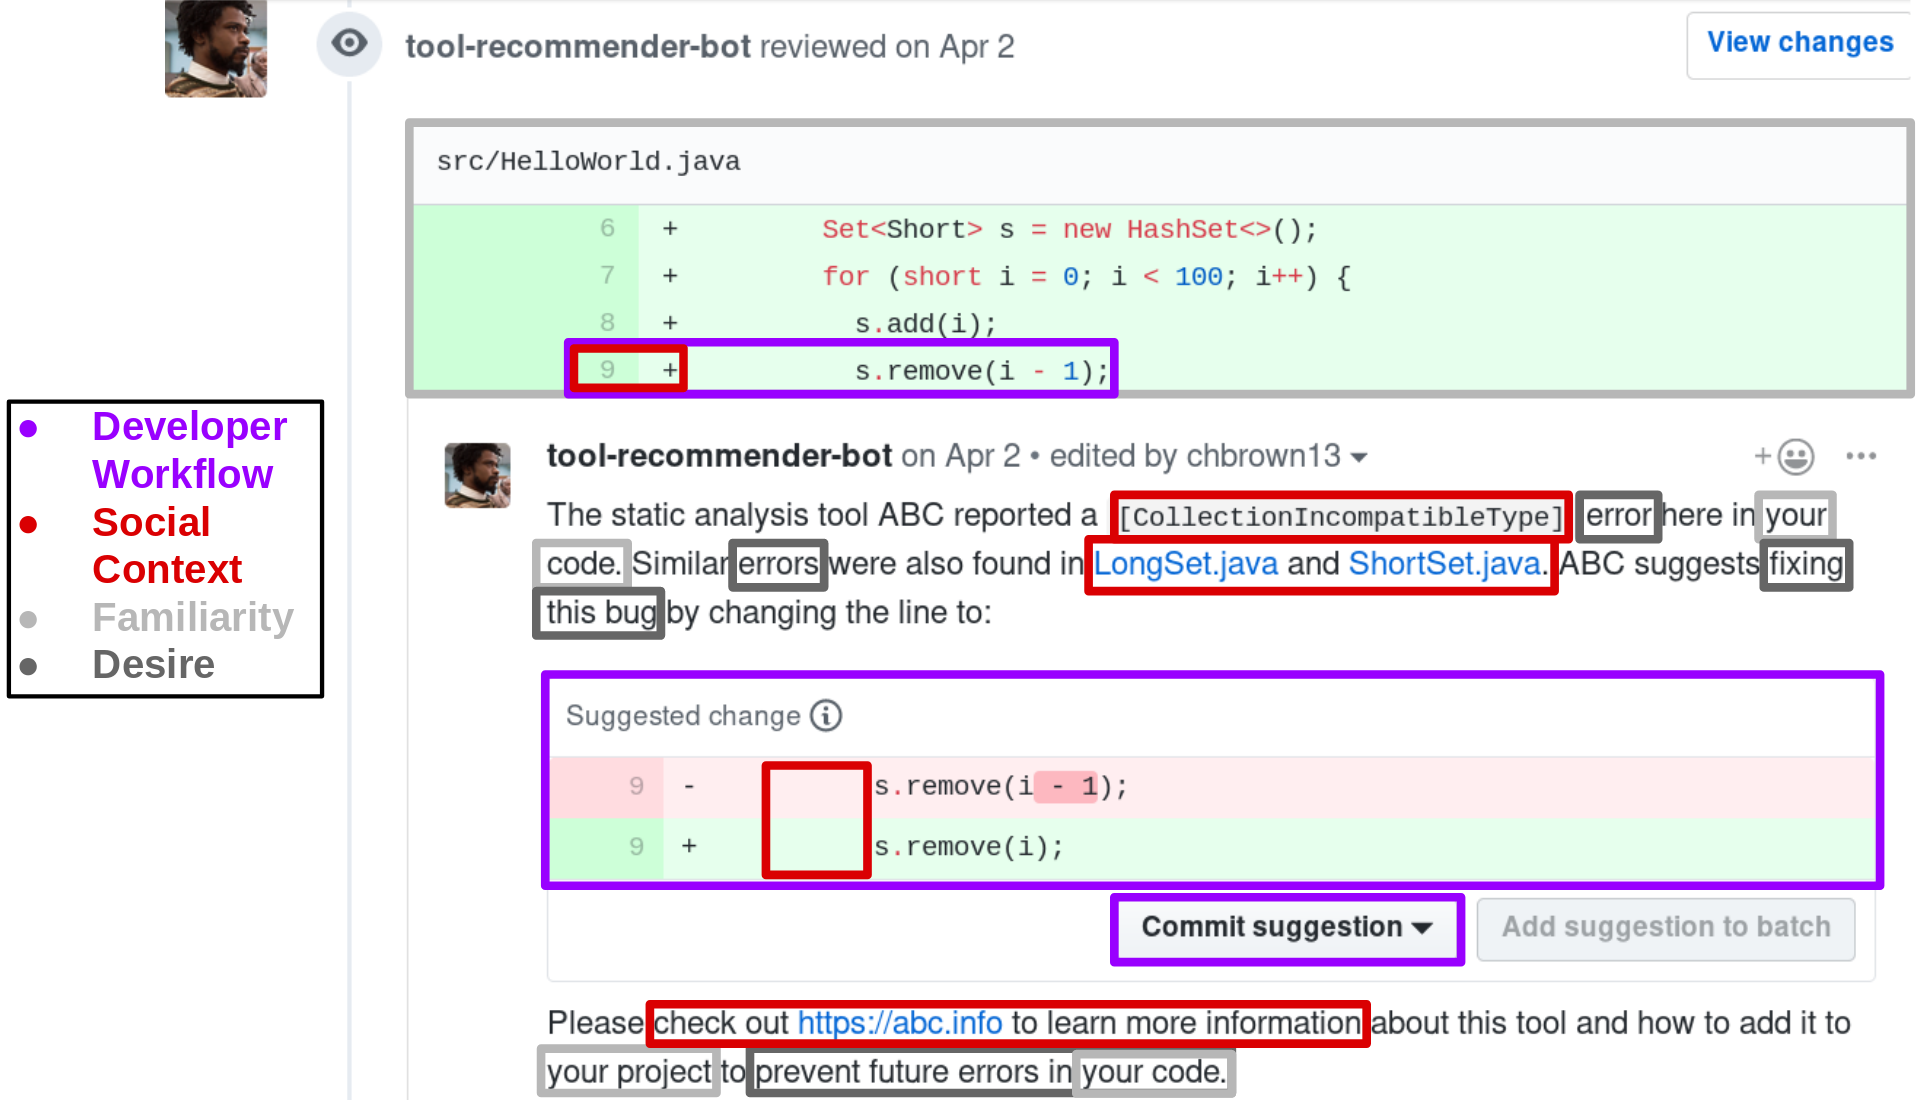
\includegraphics[width=\textwidth]{images/toolapproach.png}
% 	\caption{Prototype implementation of the framework in \TOOL}	
% 	\label{fig:approach} 
% \end{figure*}


% We iteratively modified \TOOL to use different recommendation approaches for nudging developers to adopt different software engineering tools. \TOOL uses a human-presenting GitHub account to recommend tools to developers. , and we also quickly discovered bot accounts are ineffective for recommendations after our original \TOOL~user\footnote{https://github.com/tool-recommender-bot} was flagged and disabled on GitHub for ``opening multiple unsolicited pull requests in other users' repositories" within a few hours of making recommendations at the beginning of our \tele~study. Our goal is for \TOOL~to integrate numerous recommendation approaches and make software engineering tool recommendations using the most effective nudge type(s) when developers are most receptive to adoption.

%\subsubsection{Spatial.}

%Nudge theory suggests that the placement of options in choice environments, or spatial locality, is an important factor in impacting human behavior and decision-making. For example, the director of food services for a school system with hundreds of thousands of children was able to convince students to eat healthier foods and less junk food by simply changing the arrangement of food choices in the cafeteria, i.e. placing carrots at eye-level instead of French fries. Using this strategy, the director was able to nudge students to adopt better diets and change the consumption of specific food items by up to 25\%~\cite[p.~1]{sunstein2008nudge}. 

%We hypothesize location impacts the effectiveness of recommendations to software engineers. For example, developers are more likely to ignore tool suggestions in emails compared to comments in the code. There are many examples of high spatial locality in software engineering. Most integrated development environments have built-in analyzers that highlight syntax errors at the line of code where developers introduce them. Figure \ref{fig:spatial} shows an example of an error reported by the tool  Pylint\footnote{https://www.pylint.org/}, a static analysis tool for Python. 

%\subsubsection{Temporal.}

%Research in nudge theory also suggests that timing of recommendations, or temporal locality, plays a role in influencing behavior. One instance of this is the concept of temptation, where Sunstein and Thaler categorize ``hot" and ``cold" states and note that humans are more likely to make certain decisions during hot times~\cite[p.~41]{sunstein2008nudge}. For example, a study found that simply asking people if they intend to purchase a new car within the next six months actually increased purchase rates by 35\%~\cite{morwitz1993intent}. \todo{Better example of timing}

%We examine temporal locality to determine if the timing of tool recommendations to software engineers impacts adoption. \todo{SE example}

%\subsection{Actionability}

%Nudge theory also suggests that actionability, or the ease in which humans can adopt decisions, impacts the choices people make.  

%We believe that actionability is another important factor in the outcome of recommendations to software engineers. \todo{SE example}

% \section{Tools}

This section outlines concepts for tools to develop and existing systems to observe for evaluating our approaches in making effective recommendations to software engineers.

\subsection{\TOOL}

% Prior work indicates \textit{active help systems} are more effective for providing suggestions to software users than passive help systems, which require users to deliberately seek help~\cite{FischerActiveHelp}.

% Research shows using software engineering tools can improve the quality of software and the efficiency of developers, but in reality developers rarely use them.

To evaluate approaches for making digital nudges to software engineers for development tool adoption, we developed \TOOL. We aim for researchers to be able to extend \TOOL to recommend useful tools to software engineers. Our system is designed to target developer receptivity in recommendations: the \textit{desire} of programmers to produce high-quality code and their \textit{familiarity} with a project's code base. \TOOL~is an automated recommender system designed to suggest software engineering tools to developers on GitHub\footnote{https://github.com}. We target GitHub users because the code hosting and collaboration website has millions of accounts and public repositories, as well as billions of code contributions from developers\footnote{https://octoverse.github.com/}. \TOOL~recommends development tools by integrating with projects' build configuration. With the rise of continuous integration and deployment, many projects implement build systems to automatically compile, test, and release their software more efficiently~\cite{AkondDeployment}. Integrating projects into the build allows developers to easily integrate new tools into their normal software development workflow. We iteratively modified \TOOL to use different recommendation approaches for nudging developers to adopt different software engineering tools. \TOOL uses a human-presenting GitHub account to recommend tools to developers. Prior work found that bots emulating humans are more effective than bot accounts~\cite{AmongTheMachines}, and we also quickly discovered bot accounts are ineffective for recommendations after our original \TOOL~user\footnote{https://github.com/tool-recommender-bot} was flagged and disabled on GitHub for ``opening multiple unsolicited pull requests in other users' repositories" within a few hours of making recommendations at the beginning of our \tele~study. Our goal is for \TOOL~to integrate numerous recommendation approaches and make software engineering tool recommendations using the most effective nudge type(s) when developers are most receptive to adoption.

\subsection{\SUGGS}

GitHub recently introduced a new feature that allows developers to suggest a change to a project's code modified by a user.\footnote{https://help.github.com/articles/incorporating-feedback-in-your-pull-request/\#applying-a-suggested-change} Suggestions can be utilized during pull request reviews, allowing reviewers to propose changes at the exact line of code in question and developers to easily accept or reject the change. Code reviews are another example of a software engineering action shown to improve code quality, and early feedback on the suggestion feature shows they are very popular and widely adopted by GitHub users. We plan to evaluate the effectiveness of GitHub suggestions as examples of a \location. These situated nudges already have over 100,000 uses on GitHub projects and developers are ``quick to adopt suggested changes" and integrate this feature into their code review process.\footnote{https://blog.github.com/2018-11-01-suggested-changes-update/} This research aims to examine situated nudges in the context of \SUGGS~to determine if the location of recommendations impacts the effectiveness of adoption for developers.

\subsection{nudge-bot}


\section{Experiments and Evaluations}

This section describes in progress and proposed studies to support this thesis. The bracketed text represents short names for each experiment and the text in parentheses displays the status and semester of submission.


%Peer learning is the process of acquiring knowledge and skills through interactions with colleagues. This type of collaboration is also important for increasing learning among software engineers, however it rarely occurs in industry. For example, Murphy-Hill and colleagues found that interactions between developers is the most effective mode of tool discovery, but they also occur infrequently in practice~\cite{Murphy-Hill2011PeerInteraction}. There are many ways for open source software developers to convey information to peers, and this study aims to discover the best way to increase peer learning for GitHub users. This research seeks to gather data describing how developers react to learning about new tools through recommendations from varying systems: emails, project issues\footnote{https://help.github.com/en/articles/about-issues}, pull requests\footnote{https://help.github.com/en/articles/about-pull-requests}, and suggestions\footnote{https://github.blog/changelog/2018-10-16-suggested-changes/}. Then, we conduct an in-depth analysis on the preferred method reported by participants to determine how effective and useful that feature is for learning in practice.

\subsection{[\suggT] ``Understanding the Impact of GitHub \emph{Suggested Changes} on Recommendations Between Developers" (In Submission, Fall 2019)}

\subsubsection{Motivation:} After exploring what makes recommendations effective for developers, the next step in my plan of work is to evaluate existing recommendation systems. GitHub recently introduced a new feature, \textit{suggested changes},\footnote{\url{https://help.github.com/articles/incorporating-feedback-in-your-pull-request/\#applying-a-suggested-change}} which fosters peer interactions online by allowing developers to recommend code changes to each other during code reviews through this novel system. Additionally, under the nudge theory framework, we believe GitHub suggested changes can be considered an example of a digital nudge. Suggested changes are used to encourage developers to improve code in their pull requests without providing incentives for committing suggestions or prohibiting alternative changes to improve the code. This research seeks to discover the impact of the recently introduced suggested changes feature by gathering data about the effectiveness of these suggestions, collecting feedback from developers about the new feature, and exploring how well the design of this feature generalizes to other types of recommendations. To our knowledge, this is the first study to analyze the suggested changes feature on GitHub. The results from this work provide implications to improve the effectiveness of recommendations to developers and are used to motivate the design of future automated recommender systems.

\subsubsection{Suggested Changes:} GitHub released suggested changes as a public beta feature in October 2018. This recently introduced feature allows GitHub users to recommend code changes on pull requests to software developers. Figures \ref{fig:sugg}a-c present how the suggested changes feature works. When a reviewer notices a line of code that can be improved, they can click on the plus (+) sign on the line of code in question to write a comment and create a suggestion. Then, the text box in Figure \ref{fig:sugg}a pops up for the users to enter their proposed change. Figure \ref{fig:sugg}b shows a developer typing their suggested code change for the pull request into the text box. Once the reviewer is finished with their suggestion, they can click on the ``Start a review" button to submit the suggested change. Finally, the developer who created the pull request can see the suggested change on their code, shown in Figure \ref{fig:sugg}c, and can commit, edit, or ignore the proposed modifications. Clicking ``Commit suggestion" will automatically add the change to the pull request as a new commit. This feature become very popular on GitHub, with developers ``quick to adopt suggested changes" into their workflow and totaled over 100,000 uses within weeks of the initial release, accounting for approximately 4\% of pull request review comments and 10\% of code  reviewers.\footnote{\label{SuggestBlog}\url{https://github.blog/2018-11-01-suggested-changes-update/}}

% \begin{figure*}[]
% \subfloat[Reviewer adds comment~]{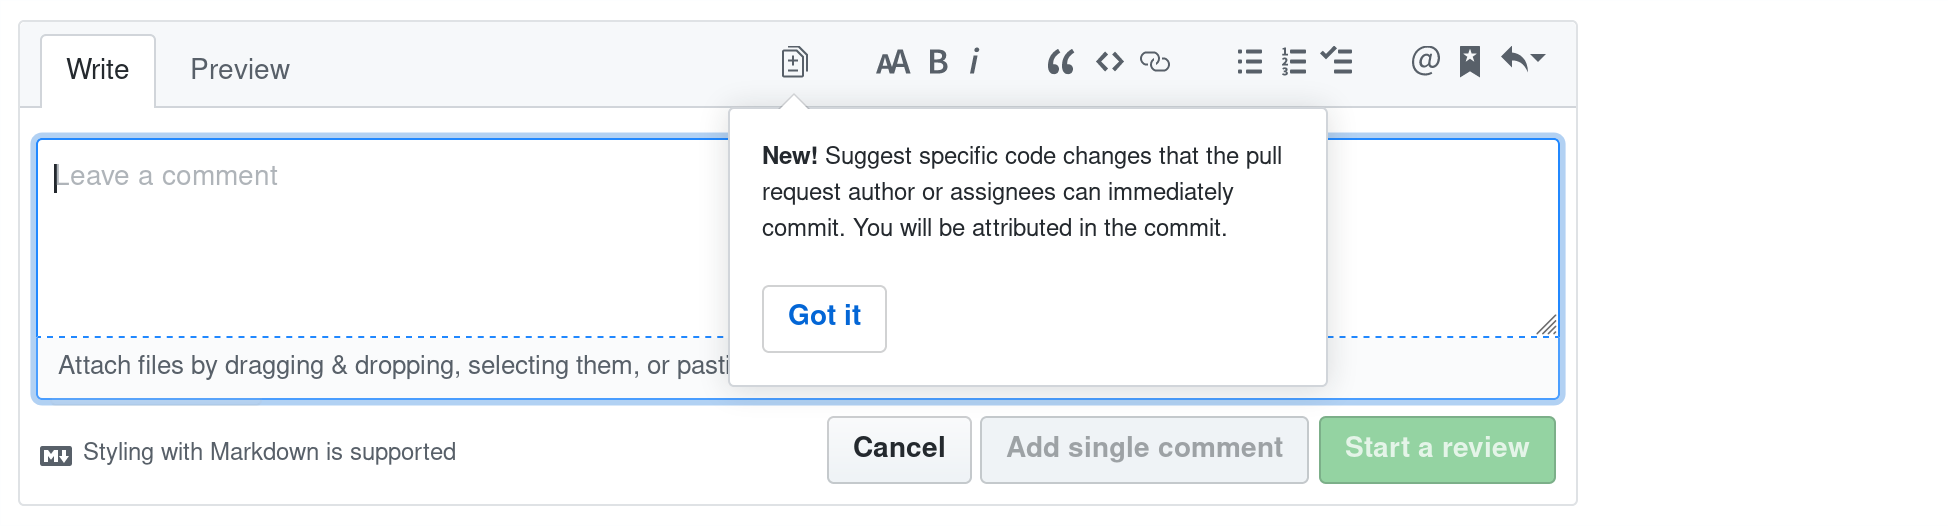
\includegraphics[width=\linewidth]{images/sugg1.png}}
% \subfloat[Reviewer suggests change~]{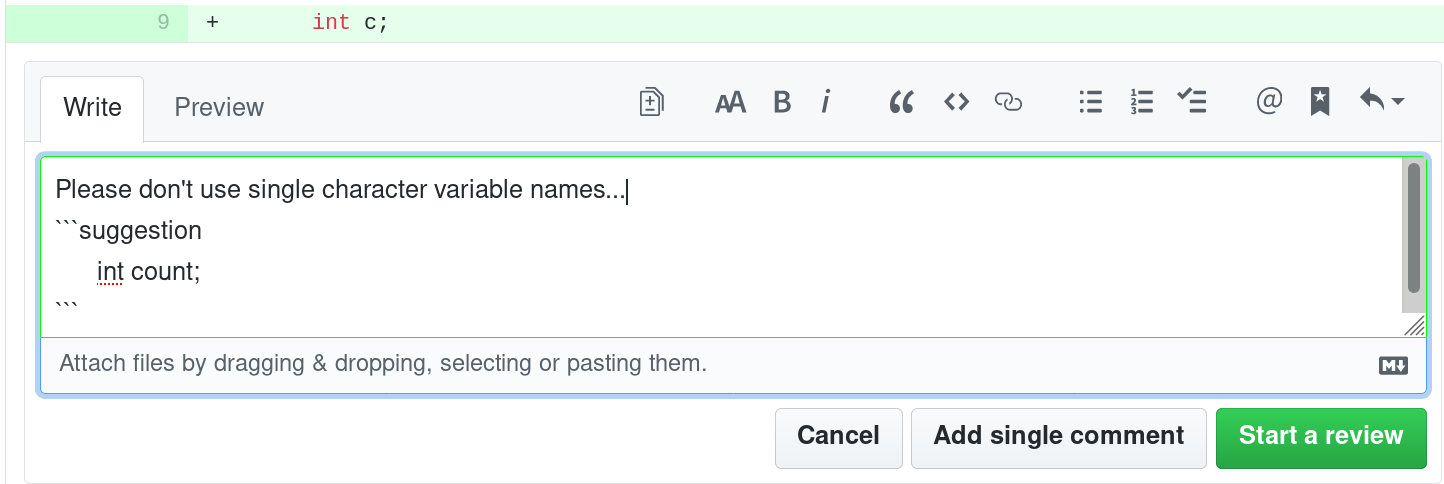
\includegraphics[width=\linewidth]{images/sugg2.png}}
% \subfloat[Developer applies suggestion]{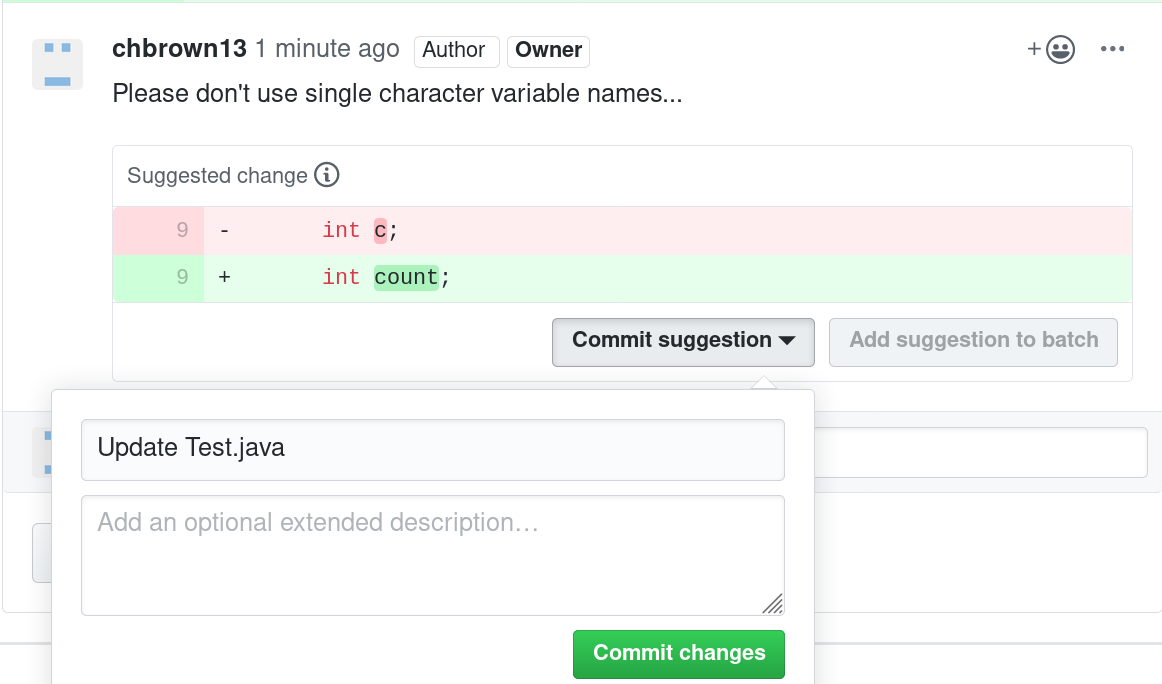
\includegraphics[width=\linewidth]{images/sugg3.png}}
% \caption{GitHub Suggested Changes example}
% \label{fig:sugg}
% \end{figure*}

\begin{figure}[]
\centering
    (a) Reviewer adds a pull request comment \\
    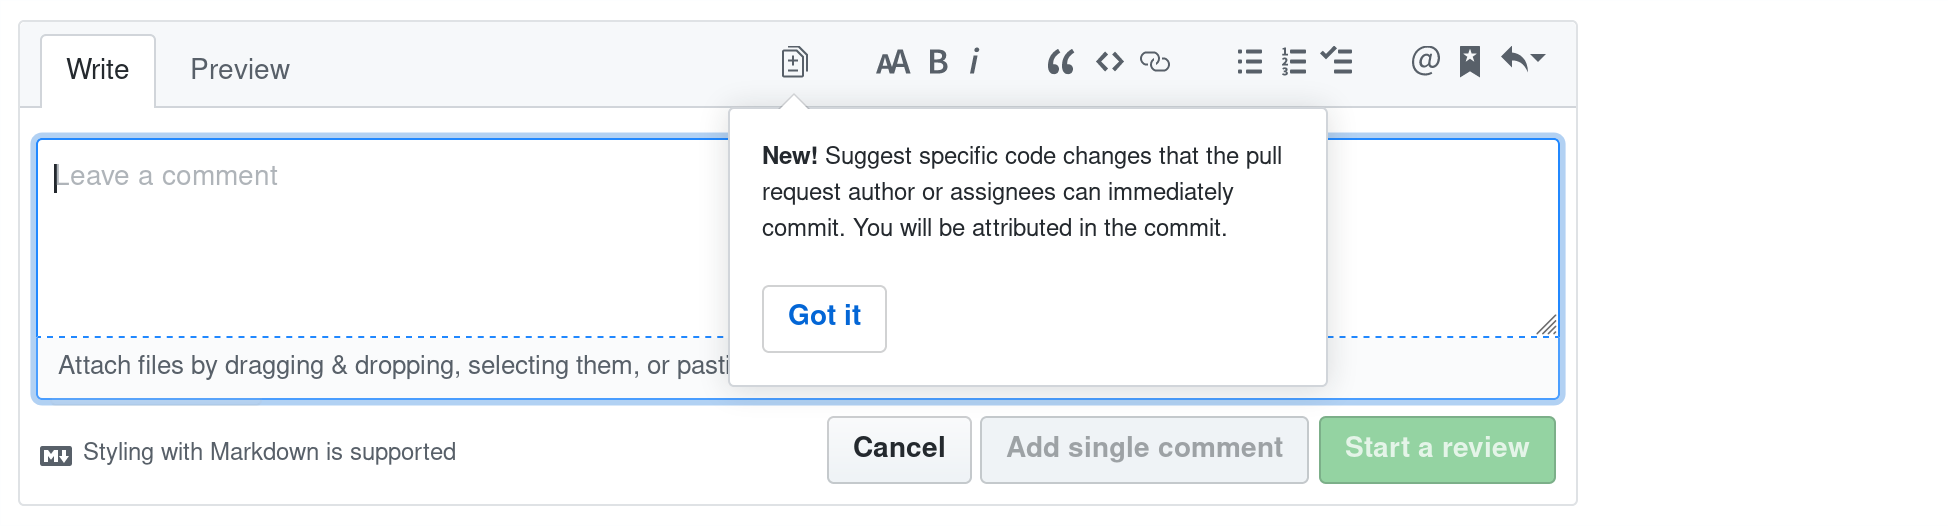
\includegraphics[width=\textwidth]{images/sugg1.png}
    (b) Reviewer suggests a code change \\
    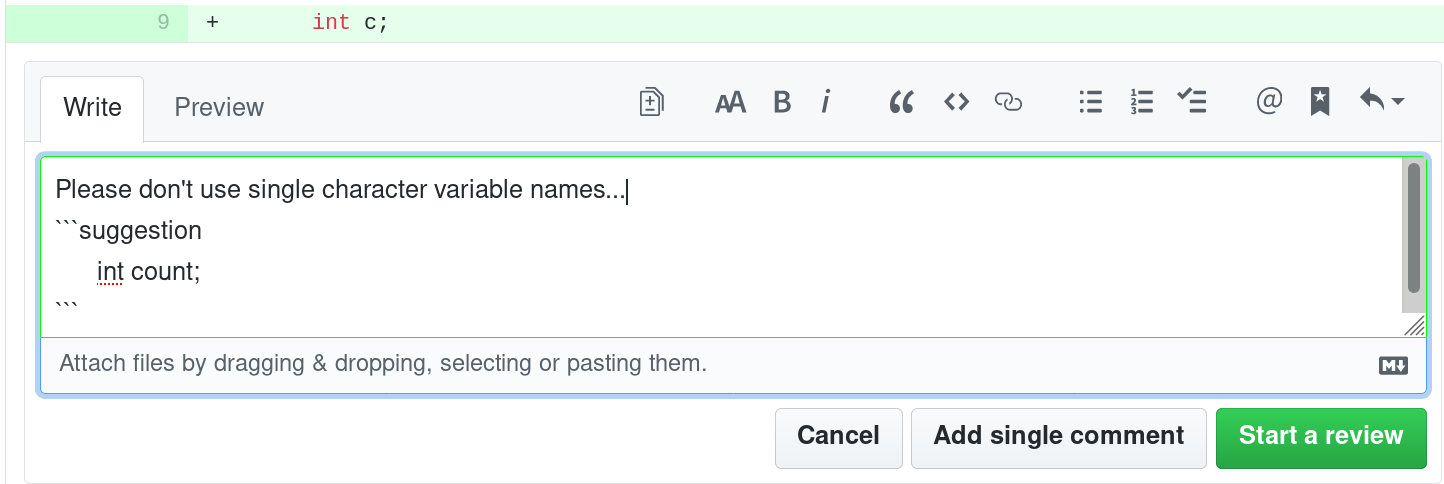
\includegraphics[width=\textwidth]{images/sugg2.png}
   (c) Developer applies suggestion from reviewer \\
    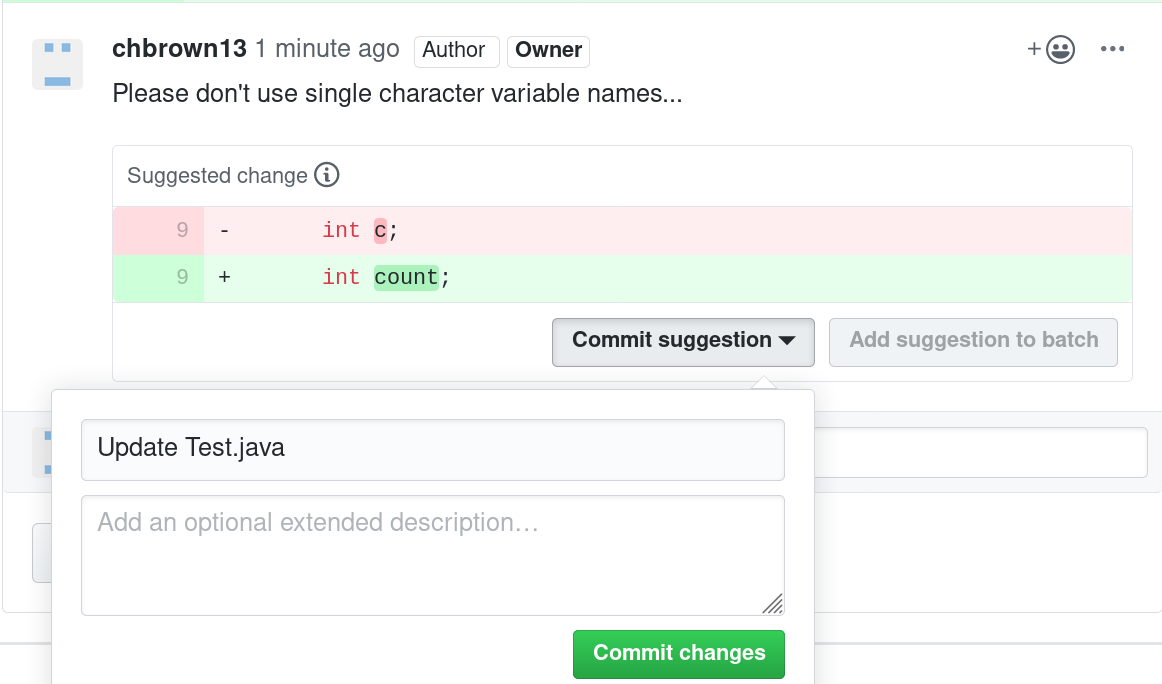
\includegraphics[width=\textwidth]{images/sugg3.png}
    \caption{GitHub Suggested Changes Example}    
    \label{fig:sugg} 
\end{figure}

\subsubsection{Research Questions:}

\begin{itemize}
    \item[\textbf{RQ1}] What suggestions do developers make with suggested changes?
    \item[\textbf{RQ2}] How effective is the suggested changes feature on GitHub?
    \item[\textbf{RQ3}] How useful is the suggested changes feature for developers?
    \item[\textbf{RQ4}] How well does the suggested changes feature generalize to other types of recommendations?
\end{itemize}

\subsubsection{Proposed Methodology:} For this research, we plan to conduct a multimethodology study divided into two phases to gather and analyze data to answer each of our research questions. \\

\subsubsection{Phase 1: \textit{An Empirical Study on GitHub Suggested Changes}} \hfill\\

The first phase of this work explores the usage and effectiveness of suggested changes on GitHub to answer the first two research questions.

\paragraph{Data Collection.}

To collect suggested changes to classify for RQ1, we developed a script to programmatically search for instances of the \sugg tag in pull request comments (See Figure~\ref{fig:sugg}b). The \sugg tag indicates that reviewer used this feature to propose a suggestion on a pull request. To gather projects and pull requests to analyze, we used the GitHub API to sort repositories by the most recently updated pull requests to compile a list of pull request with suggested changes. The script for automatically detecting uses of the suggested changes feature on GitHub pull requests is publicly available online.\footnote{\url{https://github.com/chbrown13/suggestions}}

To explore the effectiveness suggested changes, pull requests, and issues for recommendations to developers on GitHub, we mined GitHub repositories to analyze these systems. We collected pull requests and issues on the top-forked projects that have PRs with suggested changes. We analyzed the repositories with the most forks because GitHub recommends forking projects to create pull requests,\footnote{\url{https://help.github.com/en/articles/fork-a-repo}} and suggested changes require PRs to make recommendations. Additionally, our we  limited our dataset to activity after October 2018 when the suggested changes feature was introduced. To answer RQ2, we analyzed a total of 3683 suggested changes from 11869 pull request review comments, 3882 pull requests, and 3516 issues. We used two metrics to measure the effectiveness of each system: \textit{acceptance} and \textit{timing}. A list of projects used for this evaluation is available in Table~\ref{tab:projects}. 

\paragraph{Classifying types of suggested changes.}
To categorize the types of changes developers suggest with this feature, we randomly sampled 100 recently updated pull requests with an instance of the \sugg tag in the comments. A random sample was used to avoid bias from classifying suggested changes from the same GitHub users and projects. To identify categories of suggested changes, two researchers performed an \textit{open} coding by analyzing pull requests review comments with the \sugg tag and code changes recommended by developers with this feature (inter-rater agreement = 71\%, Cohen's $\kappa$ = 0.5942). The two coders then came together to discuss their results come to an agreement. Below we define and provide examples of the four identified categories for suggested changes:

\textbf{Corrective:} The corrective category refers to using suggested changes to fix issues found in the code. Software engineering research shows corrective changes are important for improving code quality. For example, Bacchelli and colleagues found that finding defects is the primary motivation for software engineers to conduct code reviews~\cite{bacchelli2013codereview}. For example, Figure~\ref{fig:categories}a presents a corrective suggested change from a reviewer on a developer's pull request. The suggestee referred to a variable as a global variable instead of a class variable, and the suggester proposes a fix by adding the \texttt{self} keyword.\footnote{\url{https://github.com/zeit/next.js/pull/7696#discussion_r302333269}}

\textbf{Improvement:} Improvement suggested changes refer to when reviewers recommend code changes to refactor or optimize a contributor's code. Developers at Microsoft reported that code improvements are the primary benefit of code reviews.\footnote{\url{https://www.michaelagreiler.com/code-reviews-at-microsoft-how-to-code-review-at-a-large-software-company/}} Additionally, further analysis by Bacchelli and colleagues revealed that, while developers reported correcting defects as the primary motivation for code reviews, code improvements were the most frequently mentioned motivation~\cite{bacchelli2013codereview}. Figure~\ref{fig:categories}b presents an instance of an improvement suggested change, where the suggester proposes improving the readability of the suggestee's code by renaming a variable from \texttt{x} to \texttt{manifest}.\footnote{\url{https://github.com/gatsbyjs/gatsby/pull/13471#discussion_r277948539}}

\textbf{Formatting:} The formatting category refers to refactoring code changes that impact the style and presentation of the code. Fixing formatting issues is also an important change to improve code. Bacchelli and colleagues reported developers also found code reviews to be useful for ensuring code styles and standards are consistent between programmers on development teams~\cite{bacchelli2013codereview}. An example of a formatting suggestion is presented in Figure~\ref{fig:categories}c.\footnote{\url{https://github.com/numba/numba/pull/4204#discussion_r310598073}} where the suggester recommends changes to fix spacing issues in the suggester's code that violate the Python PEP8 whitespace standards.\footnote{\url{https://www.python.org/dev/peps/pep-0008/#whitespace-in-expressions-and-statements}}

\textbf{Non-Functional:} Non-functional suggested changes refer to modifications reviewers recommend outside of the code. This includes suggestions to fix spelling and grammar issues or reword phrases in code documentation and comments. Non-functional changes are prevalent in software engineering, for example Beller and colleagues found that documentation changes are the most frequent type of fixes applied during code reviews for open source software~\cite{beller2014modern}. Figure~\ref{fig:categories}d presents an example of a non-functional suggested change. In this case, the suggester discovers a typo where the suggestee misspelled \textit{deserialize} in a documentation files and uses the suggested changes feature to recommend a fix for the error.\footnote{\url{https://github.com/microsoft/terminal/pull/1258#discussion_r293932790}}

\begin{figure}[]
\centering
    \textbf{(a) Corrective: \\}
    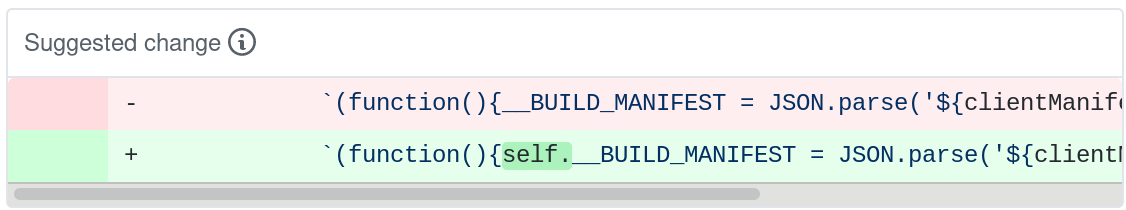
\includegraphics[width=\textwidth]{images/correct.png}
    \textbf{(b) Improvement: \\}
    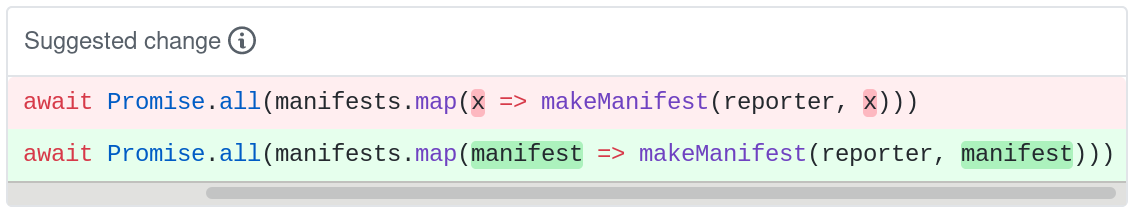
\includegraphics[width=\textwidth]{images/improve.png}
    \textbf{(c) Formatting: \\}
    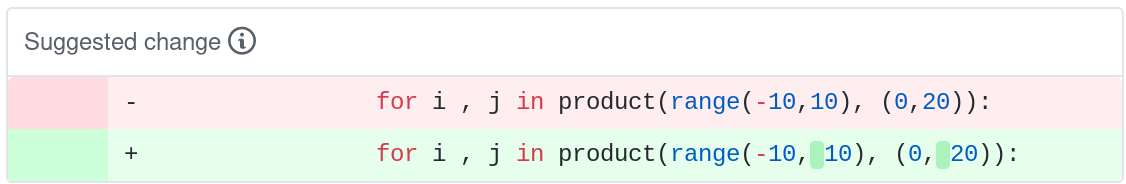
\includegraphics[width=\textwidth]{images/format.png}
    \textbf{(d) Non-Functional: \\}
    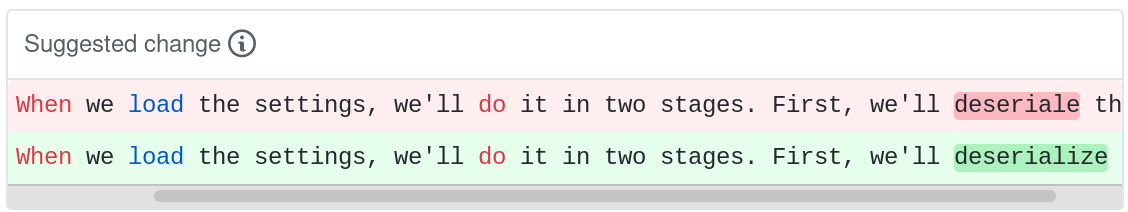
\includegraphics[width=\textwidth]{images/nonfunc.png}
    \caption{Suggested Changes Categories}    
    \label{fig:categories} 
\end{figure}

\paragraph{Determining acceptance of recommendations.}

We define acceptance as the process of users welcoming suggested changes recommended by another developer. Accepting these suggestions indicates an effective recommendation because the author trusts changes and believes it will be beneficial to the code. Research shows this concept is important in software development. For example, to emphasize the importance of acceptance in software engineering, Middleton and colleagues argue receiving code contributions from outside developers is essential for the maintenance and evolution of open source software~\cite{Middleton2018Contributions}.

Since the suggested changes feature is currently not supported by the GitHub API,\footnote{\url{https://github.community/t5/GitHub-API-Development-and/Accessing-the-new-quot-GitHub-Suggestions-quot-via-API-public/td-p/13922}} we extended the suggested changes detection script to examine commits made on pull requests with suggestions. To determine whether suggestions were accepted or rejected, our script found instances of pull requests with suggested changes. Then, it parsed review comments on the PR to extract the recommended code modifications between the \sugg tag and the ending \texttt{'''}. Finally, it checked whether the suggested line of code was present in another commit after the comment was made to the pull requests on the same file that received the suggested change. Suggested changes with lines of code that were found to be integrated in a subsequent commit on a pull request were considered accepted, otherwise they were regarded as rejected.

To determine the acceptance of pull requests, we simply used the existing GitHub status. In the pull-based software development model, accepted changes must be merged into the source code~\cite{gousios2014exploratory}. In this case, a Merged PR is considered accepted because the recommended code changes were reviewed and approved by a maintainer to be integrated into the project. For issues, the only possible statuses are Open or Closed. Thus, we were not able to automatically detect if recommendations from this system were closed to be accepted into repositories or closed to be ignored. To analyze only accepted issues with recommendations, we filtered out issues with GitHub labels \texttt{bug} and \texttt{duplicate} to avoid bug reports and multiple instances of the same issue.\footnote{\url{https://help.github.com/en/articles/about-labels}} After automatically filtering these labels, a researcher manually examined the title, description, discussion, and status of issues to code issues based on two criteria: 1) if they contain a \textit{recommendation} or \textit{no recommendation} and 2) if the recommendation was \textit{accepted} or \textit{not accepted} into the project. Accepted issues are those with recommendations that are integrated with a pull request or commit to the repository.

\paragraph{Determining timing of recommendations.}

The second metric used to determine the effectiveness of recommendations was the amount of time developers took to accept a suggestion, or acceptance time, for each system. In behavioral economics, Kocher and colleagues suggest the time to make decisions is important to the quality of choices because ``time \textit{is} money"~\cite{kocher2006time}. In software engineering, research also shows that time can impact the cost and effort required to fix bugs in code~\cite{Williams2007FaultFixTime}. To measure timing for each system, we calculated the amount of time between the creation of the recommendation and its acceptance into the repository.

For suggested changes, we measured the acceptance time as the amount of time between a reviewer commenting on a pull request with the \sugg tag until the time a subsequent commit adding the suggested line of code was created on the pull request. To measure the acceptance time for pull requests, we used the GitHub API to calculate the difference between the time from when a GitHub developer creates a pull request and when the pull request is merged into the repository by a project maintainer. After manually inspecting issues to determine they have an accepted recommendation, we used the GitHub API to determine the acceptance time for these issues by calculating the difference between the time the issue was created and the time it was closed.

\begin{table}[tbh]
\centering
\begin{tabular}{ lllrrr } \hline
  \textbf{Project} & \textbf{Primary Language} & \textbf{Forks} & \textbf{Suggested Changes} & \textbf{PRs} & \textbf{Issues} \\ \hline
 qmk/qmk\_firmware & C & 8723 & 3627 & 1997 & 290 \\
 h5bp/Front-end-Developer-Interview-Questions & HTML & 8325 & 1 & 35 & 5  \\
 Azure/azure-quickstart-templates & PowerShell & 7743 & 2 & 921 & 147 \\
 firebase/quickstart-android & Java & 5603 & 2 & 91 & 124 \\ 
 mavlink/qgroundcontrol & C++ & 1584 & 4 & 402 & 267 \\
 qgis/QGIS & C++ & 1516 & 47 & 436 & 2683 \\

\end{tabular}
\caption{RQ2 Study Projects}
\label{tab:projects}
\end{table}

\subsubsection{Phase 2: \textit{Developer Feedback on Suggested Changes}}

The second phase consisted of a survey and user study to answer the last two research questions on the usefulness and generalizability of GitHub suggested changes.

\paragraph{Data Collection.}

To determine the usefulness of suggested changes, we surveyed developers who interacted with the feature on GitHub. Surveys were emailed to users with publicly available email addresses who either received or made a suggestion on a pull request within the last six months. Our survey asked users how useful they found the this feature using a 5-point Likert scale as well as free response questions to provide details on what specifically they find useful or not useful about the system and how it is integrated it into their project.

To answer RQ4, we conducted a user study to examine applying the suggested changes feature to tool recommendations. We recruited 14 professional software developers, presented in Table~\ref{tab:participants}, to participate in this study. The participants averaged 5 years of industry experience in various roles such as Software Engineer, Software Developer, Quality Engineer, Consultant, Data Migration Consultant, Support Specialist, User Researcher, and Technical Test Lead. Additionally, all participants were at least somewhat familiar with GitHub. We conducted a think aloud study with a semi-structured interview and audio and screen recorded all sessions to collect feedback from developers on how well the suggested changes feature translates to software engineering tool recommendations. 

\paragraph{Determining usefulness of suggestions.}

We emailed surveys to a total of 570 GitHub users who interacted with suggested changes and received 39 responses (7\% response rate).  Throughout the remainder of this paper, we use the \see- prefix to describe a \textit{suggestee}, or a contributor who received a suggested change on their pull request, and the \ser- prefix to indicate a \textit{suggester}, or a reviewer who made a comment with the suggested changes feature on a pull request. We aggregated the Likert scores to examine the overall usefulness, then two experts \textit{open} coded the open-ended responses from developers on the useful (72\%, $\kappa$ = 0.6828) and unuseful (77\%, $\kappa$ = 0.7125) aspects of suggested changes. The researchers discussed derived categories and came to a consensus on themes found in comments. To resolve disagreements in coding statements, the first author acted as the tie-breaker. The primary inconsistencies in coding came from determining the existence of multiple themes since responses from developers could span more than one category.

\paragraph{Determining the generalizability of recommendations.}


To determine the impact of suggested changes on tool recommendations, we asked participants to interact with sample recommendations from a suggested change, pull request, issue, and email. Participants were asked to provide a Likert-scale ranking on how likely they would adopt the tool and to discuss what they like and dislike about each system as well as provide insight into what makes tool recommendations effective in general. Figure~\ref{fig:tool} presents an example of the prototype suggested change recommendation system, using the feature to suggest a fix for a bug reported by static analysis output and recommend a tool for developers to find and prevent errors in the future. Staged recommendations for pull requests, issues, and emails contained similar text suggesting tools to participants from each system. To analyze feedback on this design, we aggregated the Likert scores and open-ended feedback from participants. For the rest of this paper, user study participants are indicated with a P-prefix. We transcribed and analyzed recordings of sessions to present feedback from developers on receiving tool recommendations with suggested changes.

\begin{table*}[]
\centering
\begin{tabular}{ lrlll } \hline
  \textbf{ID} & \textbf{Experience (years)} & \textbf{GitHub Familiarity} & \textbf{OSS Contribution Frequency} & \textbf{Tool Usage Frequency} \\ \hline
 % P0.1 & PhD student & 3 & Moderate & Very Frequently \\  
 % P0.2 & PhD student & 0.5 & Moderate & Rarely \\ 
 P1 & 30 & Very Familiar & Occasionally & Very Frequently \\  
 P2 & Less than 1 & Moderately Familiar & Never & Never \\ 
 P3 & Less than 1 & Very Familiar & Rarely & Moderately Frequent \\  
 P4 & 8 & Very Familiar & Very Frequently & Very Frequently \\ 
 P5 & 10 & Familiar & Rarely & Moderately Frequent \\
 P6 & 5 & Moderately Familiar & Occasionally & Very Frequently \\
 P7 & 6 & Familiar & Frequently & Very Frequently \\
 P8 & 6 & Familiar & Very Frequently & Very Frequently \\
 P9 & Less than 1 & Moderately Familiar & Occasionally & Very Frequently \\
 P10 & 1 & Moderately Familiar & Occasionally & Very Frequently \\
 P11 & 3 & Familiar & Very Frequently & Very Frequently \\
 P12 & 3 & Familiar & Rarely & Very Frequently \\
 P13 & 1 & Moderately Familiar & Never & Never \\
 P14 & 1 & Moderately Familiar & Never & Frequently \\
 \hline
 
\end{tabular}
\caption{RQ4 User Study Participants}
\label{tab:participants}
\end{table*}

\begin{figure}[]
	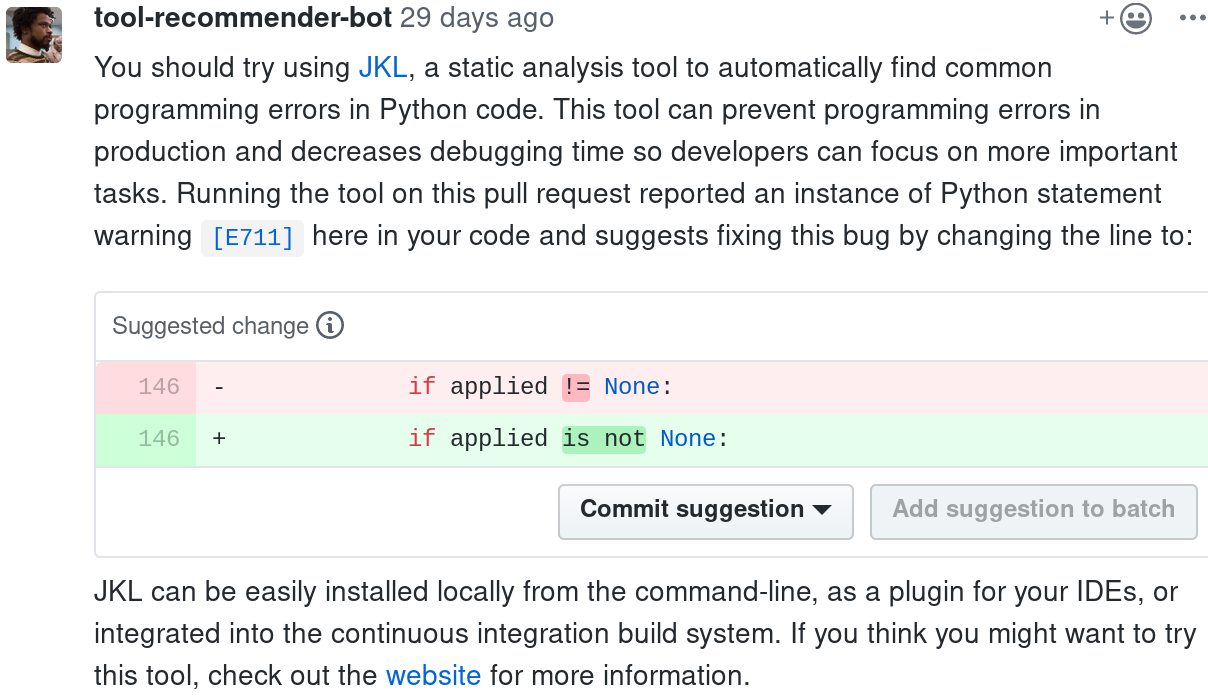
\includegraphics[width=\textwidth]{images/auto_suggest.png}
	\caption{Mock Recommender system with suggested changes}	
	\label{fig:tool} 
\end{figure}


\subsubsection{Expected Results:} From this evaluation, I expect to gain insight into the effectiveness of the GitHub suggested changes feature in recommendations between developers. For RQ1, we hypothesize that suggested changes are useful for recommending a wide variety of code changes. For RQ2, we hypothesize suggested changes are as effective as other systems for recommendations between users on GitHub. For RQ3, we expect users find this new feature very useful for suggesting and receiving code change recommendations. Finally, for RQ4 we believe the design of this system can generalize to other types of recommendations and is preferred by software developers for recommending static analysis tools. The results of this evaluation were submitted for publication to the 2020 International Conference on Software Engineering (ICSE 2020).\footnote{\url{https://conf.researchr.org/home/icse-2020}}

% \paragraph{RQ1: Usage.}

% \begin{table}[H]
% \centering
% \begin{tabular}{ |c|c|c|} \hline
%   & \textbf{\textit{n}} & \textbf{Percentage} \\ \hline
%  Non-Functional &  36 & 36\% \\ \hline
%  Improvement & 34  & 34\% \\ \hline 
%  Corrective &  16 & 16\% \\ \hline
%  Formatting & 14 & 14\% \\ \hline
% \end{tabular}
% \caption{Suggested Change Categories}
% \label{tab:rq1}
% \end{table}

% We discovered that most suggested changes to developers were recommendations for non-functional changes. Table~\ref{tab:rq1} presents our findings for each category from 100 randomly sampled uses of the suggested changes feature on GitHub. While non-functional changes were the most frequent type of changes recommended with this feature, we found that suggested changes are also useful for recommending a wide variety of code modifications to developers during reviews. 

% \paragraph{RQ2: Effectiveness.}

% Our results suggest that pull requests are still the primary method for GitHub developers to accept recommendations. Table~\ref{tab:accept} presents our results for acceptance for each system. Using a chi-square test to analyze the outcome of recommendations for each group, we found that the difference in acceptance was statistically significant for suggested changes, pull requests, and issues ($\chi^2$ = 1128.7155, p < .00001, $\alpha$ = .05). Approximately 78\% of PRs we analyzed were merged into repositories compared to 69\% of suggested changes and only 17\% of issues. While suggested changes are a relatively new feature, many projects have already adopted the pull-based model for software development on GitHub~\cite{gousios2014exploratory,  gousios2015work}.

% \begin{table}[H]
% \centering
% \begin{tabular}{ |c|c|c|} \hline
%   & \textbf{\textit{n}} & \textbf{Rate} \\ \hline
%  suggestions & 2554 & 69.3\% \\ \hline 
%  pull requests & 3044 & 78.4\% \\ \hline
%  issues & 133 & 17.2\% \\ \hline
% \end{tabular}
% \caption{Acceptance Rate}
% \label{tab:accept}
% \end{table}

% For timing, we found that recommendations for suggested changes are accepted into repositories almost twice as fast as pull requests, while issues remain much less effective. Table~\ref{tab:time} presents the average acceptance time for each type of recommendation. Using the Kruskal-Wallis test to analyze the time data, we found a significant difference in the amount of time taken to accept a recommendation for each system (Kruskal-Wallis = 391.844102, \textit{p} < .0001, $\alpha$ = .05). This indicates that developers are able to make a decision on whether to accept or reject recommendations using suggested changes much faster than with pull requests or issues. Shorter acceptance times are useful in software engineering to help reduce \textit{fault fix latency}, or the amount of time a defect exists in code~\cite{Layman2007FaultFixTime}. This can prevent wasted time, effort, and costs to fix latent bugs during the software development process.

% \begin{table}[H]
% \centering
% \begin{tabular}{ |c|c|c|c| } \hline
%   & \textbf{Average (days)} & \textbf{Median (days)} \\ \hline
%  suggestions & 2.9 & 0.3 \\ \hline 
%  pull requests & 5.0 & 0.8 \\ \hline
%  issues & 28.5 & 2.6 \\ \hline
% \end{tabular}
% \caption{Acceptance Time}
% \label{tab:time}
% \end{table}

% To further understand the impact of suggested changes, we observed their impact on the effectiveness of pull requests themselves. We collected results on the acceptance and timing of pull requests with and without suggestions. The findings from this analysis are presented in Table~\ref{tab:acceptPR}. We found that that pull requests with suggested changes were accepted significantly more often than pull requests without them ($\chi^2$ = 6.1296, \textit{p} = 0.013294, $\alpha$ = .05). However, we also surprisingly discovered that pull requests with suggested changes take significantly longer to be accepted than those without (Wilcoxon, \textit{p} < .0001, $\alpha$ = .05). This may be due to the fact that, while individual suggested changes are quickly accepted by developers, one pull request often has multiple changes suggested. In the data collected study the influence of suggested changes on PRs, we observed each pull request had an average of six comments with suggested changes. This shows that pull requests with suggested changes are more complex. While this feature helps resolve problems in code reviews and eventually get pull requests accepted, they also add more time to code inspections.

% \begin{table}[H]
% \centering
% \begin{tabular}{ |c|c|c|c| } \hline
%   \textbf{Pull Requests} & \textbf{\textit{n}} & \textbf{Acceptance} & \textbf{Timing (days)} \\ \hline
%  with suggestions & 559 & 79.8\% & 8.88 \\ \hline 
%  without suggestions & 3323 & 78.2\% & 4.34 \\ \hline
% \end{tabular}
% \caption{Pull Request Data}
% \label{tab:acceptPR}
% \end{table}

% \paragraph{RQ3: Usefulness.}

% Figure~\ref{fig:usefulness} presents the Likert results on how useful the 39 survey respondents found the suggested changes feature. No GitHub users who interacted with this feature responded that it was Not at All Useful. Meanwhile, 95\% of suggestees and 76\% of suggesters responded they believe the suggested changes feature is Useful or Very Useful. This suggests that GitHub users find this system useful for both receiving recommendations from peers as well as sharing knowledge and making suggestions to colleagues on GitHub.

% \begin{figure}
% \begin{tikzpicture}
% \begin{axis}[
%     xbar stacked,
%     ytick=data,
%     axis y line*=none,
%     axis x line*=bottom,
%     tick label style={font=\footnotesize},
%     legend style={font=\footnotesize},
%     label style={font=\footnotesize},
%     xtick={0,5,10,15,20,25},
%     width=\textwidth,
%     bar width=6mm,
%     xlabel= Number of Participants,
%     yticklabels={Not at All Useful, Somewhat Useful, Moderately Useful, Useful, Very Useful},
%     xmin=0,
%     xmax=25,
%     area legend,
%     y=8mm,
%     enlarge y limits={abs=0.625},
% ]
% % Suggesters
% \addplot[fill=lightgray] coordinates
% {(0,0) (1,1) (3,2) (7,3) (6,4)};
% % Suggestees
% \addplot[fill=black] coordinates
% {(0,0) (0,1) (1,2) (14,3) (7,4)};
% \legend{Suggester, Suggestee}
% \end{axis}  
% \end{tikzpicture}
% \caption{Survey Results}
% \label{fig:usefulness}
% \end{figure}

% To further examine the usefulness of suggested changes, we asked survey participants to provide open-ended responses describing what they find useful or not useful about this feature. Table~\ref{tab:useful} presents the number of comments observed in feedback derived from developers. A large majority of feedback from programmers consisted of complaints about desired features currently not supported by GitHub suggested changes. We combined comments that refer to functionality out of scope for suggested changes, such as multi-line suggestions and squashing commits, as \textit{unsupported features}. We found the inability to support advanced features weighed on participants' overall perceived value of the feature. For example, \ser11, who ranked the suggested changes feature as Somewhat Useful, responded they desired a ```force push' option, because that matches our workflow". For feedback on the current implementation of the suggested changes feature, 15 developers found it inconvenient to integrate this system with their existing tools and processes. For instance, \see16 complained `their `CI process doesn't work on suggested change[s]".

% The main feedback we discovered on the usefulness of suggested changes is that they are effective for communication between developers. This category refers to the understanding and clarity in transferring knowledge between peers, and 17 comments mentioned this feature allowed developers to share and understand feedback clearly during code reviews. For example, \ser12 responded ``I find it *so* useful. It completely removes all ambiguity about what I'm asking for". Another key benefit of suggested changes is the timing of this feature, with 11 participants noting it ``accelerates getting pull requests accepted" (\see4) and ``speeds up the review process" (\see18). While programmers applauded the clarity and speed of suggested changes and disapproved of their lacking functionality and poor integration, they had mixed consensus on the actionability and conciseness of this feature. 


% \begin{table}[H]
% \centering
% \begin{tabular}{ |c|c| } \hline
%  \textbf{Useful} & \textbf{\textit{n}} \\ \hline
%  Communication & 17 \\ \hline
%  Conciseness & 13 \\ \hline 
%  Timing & 11 \\ \hline
%  Ease of Use & 7 \\ \hline
%  Actionability & 6 \\ \hline
%  Location & 5 \\ \hline
%  Scalability & 4 \\ \hline
%  Did Not Answer & 4 \\ \hline
%  Code & 3 \\ \hline
%  Attribution & 1 \\ \hline
% \end{tabular}
% \begin{tabular}{ |c|c| } \hline
%  \textbf{Unuseful} & \textbf{\textit{n}} \\ \hline
%  Unsupported Features & 24 \\ \hline 
%  Integration & 15 \\ \hline
%  Actionability & 12 \\ \hline
%  Conciseness & 6 \\ \hline
%  Formatting & 4 \\ \hline
%  Did Not Answer & 3 \\ \hline
%  Nothing & 3 \\ \hline
%  Mentoring & 1 \\ \hline
%  Rejection & 1\\ \hline
%   & \\ \hline
% \end{tabular}
% \caption{Number of Comments for Feedback Categories}
% \label{tab:useful}
% \end{table}

% \paragraph{RQ4: Generalizability.}

% Based on the results from the user study, we found that the suggested changes feature was the preferred tool recommendation method by developers who participated in our study. Table~\ref{tab:rank} shows the average and median Likert scores representing the likelihood participants would adopt the tool from each method of recommendation. The Kruskal-Wallis test was used to statistically measure differences in developer responses to tool recommendations from suggested changes, pull requests, issues, and email. We found a significant difference in likelihood of adoption provided by participants for the four systems for recommendations (Kruskal-Wallis, \textit{p} = .00079, $\alpha$ = .05). This shows that the design of the suggested changes feature is not only useful for suggesting code modifications during code reviews, but can also apply to software engineering tool recommendations to developers.

% \begin{table}[H]
% \centering
% \begin{tabular}{ |c|c|c| } \hline
%   & \textit{\textbf{Average Score}} & \textit{\textbf{Median}} \\ \hline
%  Suggestions & 4 & 4 \\ \hline 
%  Pull Requests & 3.71 & 4 \\ \hline 
%  Issues & 2.86 & 3 \\ \hline 
%  Email & 2.36 & 2 \\ \hline 
% \end{tabular}
% \caption{Effectiveness for Developers}
% \label{tab:rank}
% \end{table}

% The user study also consisted of a semi-structured interview, where we were particularly interested in gaining insight into using suggested changes for suggesting tools and improving developer recommendations. We used this feedback as well as developer survey responses on the usefulness of suggested changes to motivate the four design principles for overcoming barriers to peer interactions and improving automated recommendations to software developers based on the suggested changes feature: \textit{social recommendations}, \textit{user-driven communication}, \textit{actionable recommendations}, and \textit{receptive choice architecture}. The results of this study have been submitted for publication at the 2020 International Conference on Software Engineering (ICSE).


\subsection{[\nudgeT] ``Nudging Student Towards Better Software Engineering Behaviors" (Proposed, Spring 2020)}

\subsubsection{Motivation:}

So far, my work has shown that peer interactions are useful because of their emphasis on user receptiveness~\cite{VLHCC} and a naive bot is ineffective for making suggestions to developers~\cite{BotSE}. Thus, we propose using nudge theory to target the receptivity of software engineers and improve automated recommendations for developer actions. To understand the impact of implementing automated recommendations as digital nudges, we plan to implement and evaluate a novel recommendation approach in a new system: \TOOL. While \tool used the \naive approach to recommend static analysis tools, we aim to enhance \TOOL by incorporating our conceptual framework in addition to design implications from the results of the \sugg study examining an existing system that can be considered a digital nudge. To evaluate this system, we plan to examine how recommendations from \TOOL improve the decision-making and behavior of students in a college-level software engineering course. While research shows that automation is useful to help with grading and teaching in introductory computer science courses~\cite{singh2013automated} and providing feedback to students~\cite{hu2019feedback}, there is little to no work exploring the use of automated recommendations to improve student behavior. We aim to show that this new system can improve student behavior in software engineering education and that the results from this evaluation can correlate to software engineers in industry.

\subsubsection{Software Engineering Education:} Research suggests improvements are needed for software engineering education and the future of the software industry. The ACM notes that there is a ``crisis" in Computer Science Education that will result in necessary computing-related jobs going unfilled~\cite{emptyfailure}. Furthermore, even though the computer science major is one of the most popular fields of study at universities, it also has a very high attrition and failure rate~\cite{beaubouef2005high}. For software engineering education, a subset of computer science, researchers have explored problems with effectively preparing students for industry. Jazayeri outlines challenges of teaching software engineering and provides ideas for a new curriculum and skills to educate successful software engineers~\cite{jazayeri2004education}. Furthermore, Devadiga argues that topics taught in school are often unrelated to industry practice and suggests merging with startups to improve SE education~\cite{devadiga2017software}. Additionally, Heckman and colleagues present ``the good, the bad, and the ugly" of teaching software engineering to students using an open source software system~\cite{Heckman2018Itrust}. Several issues they found include delayed feedback, group dynamics, high workload, and aggressive scheduling. We aim to improve on these problems in software engineering education by nudging students to adopt useful developer actions and make better decisions in the context of software engineering with automated feedback on course projects.

\subsubsection{Research Questions:}

\begin{itemize}
    \item[\textbf{RQ1}] How do digital nudges influence software engineering student behavior?
    \item[\textbf{RQ2}] How do digital nudges impact software engineering student performance?
\end{itemize}

\subsubsection{Proposed Methodology:}

To evaluate integrating nudge theory into developer recommendations, we plan to conduct a mixed-methods research study.

\paragraph{Data Collection.} The data for this evaluation will be collected from the undergraduate (CSC 326) Software Engineering course at North Carolina State University. First, we will analyze data from mining GitHub repos for final projects from previous semesters of CSC 326. This will help us determine which project milestones to nudge for as well as when to nudge. In this stage, we will collect information from past repositories such as project grades, submission times, amount of time to complete various milestones, and code contributions by each group member. While the project requirements change for the team project each semester, each iteration of the class will have similar milestones to complete every year. Additionally, we hope to conduct a pilot study to test \TOOL and develop our study design during the final project for CSC 326 this semester.

After examining projects from prior semesters to determine the best time to nudge, we plan to mine repositories for the CSC 326 final project in Spring 2020 to answer our research questions. Participants will be volunteers in software engineering groups from the class who opt-in to receiving notifications from a bot. We plan to gather quantitative data based on student behaviors and performance on the final project as well as the acceptance of recommendations. Additionally, we will collect qualitative data on by surveying students to learn about their perception of the recommendations from our automated system.

\paragraph{Implementing \TOOL.} To build our new \TOOL recommender system, we used the Source Optics code activity analysis platform.\footnote{\url{https://sourceoptics.io}} Source Optics is a framework that allows users to observe and mine information for repositories presented in a browser. Our bot will be built on top of this platform to encourage developers to adopt better behaviors based on monitored activity. We plan to design our bot to incorporate results from the prior work to address our conceptual framework for making effective recommendations to developers. In our evaluation, \TOOL will send notifications to students encouraging to adopt better development behaviors on their project by emailing individuals based on their behavior for contributing to the team's repository. The input to the system will be a YAML file mapping project milestones with deadlines and containing other information such as project team members and contact information. \TOOL will be deployed on Jenkins servers used for the CSC 326 course. Our goal is for software engineering educators to be able to customize \TOOL and integrate it into their SE courses and projects, and for software engineering researchers to be able to extend this system to recommend useful actions to developers contributing to open source software. The code for \TOOL will also be publicly available online.\footnote{\url{https://github.com/chbrown13/nudge-bot}}

\paragraph{Defining student behaviors.} To answer RQ1, we will observe the following concepts to measure student behavior.

\textit{1) Project Milestones} For each project milestone, we plan to nudge students who have not started on specific tasks with an approaching deadline to encourage them to begin. Beaubouef and colleagues note that poor project management is a hindrance for computer science students. This also applies to professional software engineers. For example, prior work suggests that the amount of time a pull request remains open impacts its status in a repository~\cite{yu2015wait}. Thus, one way to minimize ignored stale and incomplete contributions for projects is to automatically nudge developers to address open pull requests. To support project management for students and improve their behaviors, we plan create digital nudges for milestones such as the following:

\begin{itemize}
    \item creating a project wiki page
    \item closing open pull requests
    \item closing open issues
    \item creating unit tests
    \item static analysis feedback
    \item test coverage remains at least 70\%
\end{itemize}

The complete list of milestones for \TOOL will be finalized after collecting data from previous semesters and piloting our system this semester. More details and information on the milestones for the final project in CSC 326 this semester is available on the course webpage.\footnote{\url{https://pages.github.ncsu.edu/engr-csc326-staff/326-course-page/team-project/}}

\textit{2) Collaboration} Another behavior we aim to improve is teamwork between team members. Williams and colleagues found that pair learning and collaboration is beneficial for software engineering education~\cite{williams2000effects}. However, enforcing student collaboration is difficult and research also shows that issues with group dynamics is a challenge in teaching software engineering~\cite{Heckman2018Itrust}. An example of this is the case where one student writes most of the code for a project where another may slack off and do very little work. This problem also exists in the software engineering. Research shows collaboration between developers is vital for software engineering~\cite{whitehead2007collaboration}. However, Agrawal and colleagues examined ``hero" projects, where 80\% of contributions are made by 20\% of developers, and found that this practice is very common in both open source and enterprise software development~\cite{Agrawal2018Hero}. To improve on this behavior in the context of student projects, we plan to nudge students who have not recently contributed to their repository (i.e. made a commit) and encourage non-performing developers to participate with the team.

\paragraph{Defining student performance.}

To answer RQ2, we define student performance as the amount of \textit{time} needed to complete the project and the final \textit{grade} of the project. For time, we aim to discover if nudging developers to start and complete milestones sooner will impact the overall amount of time needed to finish the project. Professional software engineers are often poor at estimating time to complete projects and fall behind schedule. Beaubouef and colleagues note that this poor project management also exists for students completing computer science class projects. To encourage students to submit deliverables for the final CSC 326 project on time, there is a 10\% deduction penalty for late submissions.

In SE education, a grade indicates the overall quality of the project. In this course, student grades for the final projects are determined by real-world software engineering quality metrics: Technical Deliverables (i.e. meeting requirements, test plan, design plan, and a demo), Technical Processes (i.e. GitHub repository setup, Jenkins builds, issue tracking, bug reporting, and using branches), Project Management (i.e. project management plan, agile development stories, documentation, team check-ins, and iterations), Team Collaboration (i.e. team contributions, number of commits, and peer evaluation) and Peer Review (i.e. code reviews).\footnote{\url{https://pages.github.ncsu.edu/engr-csc326-staff/326-course-page/team-project/#grade-categories}} Additionally, Beaubouef and colleagues note that poor grades is one aspect of introductory computer science classes that discourages students and leads them to drop the major and suggest that better grades could result in increased retention~\cite{beaubouef2005high}. We aim to determine if digital nudges to improve student behavior and decision-making while completing their final project can improve grades.

\subsubsection{Expected Results:}

We hypothesize that integrating concepts nudge theory into automated recommendations to software engineering students will improve their behavior while working on teams to complete a development project. Specifically, we believe that \TOOL can improve developer behavior by: 1) increasing the completion of developer actions such as adding documentation, writing tests, commits, addressing issues and pull requests, etc. 2) increasing collaboration and participation among project teams, 3) reducing the amount of time to complete the project by encouraging students to start and finish milestones earlier, and 4) increasing the overall software quality and student grades for the team project.

\section{Related Work}

My research is based on prior work that explores making recommendations to developers and technical approaches to increasing software engineering action adoption.

\subsection{Developer Recommendations} 

Prior work has investigated different methods for making effective recommendations to software developers. One such method is in-person interactions between with colleagues, which research suggests is the most effective way to make suggestions to software engineers. Murphy-Hill explored seven methods software engineers learn about new development tools and found that \textit{peer interactions} were the most effective~\cite{Murphy-Hill2015HowDoUsers}. Additionally, Cockburn and Williams suggest that collaboration occurring pair programming is useful for saving time and money in addition to  improving developer work satisfaction, design quality, code reviews, problem solving abilities, learning, team building, communication, and project management within an  organization~\cite{WilliamsPairProgramming}. Likewise, Maaleej also analyzed peer debriefings, or discussions between developers, and found that these peer interactions are effective for improving code comprehension~\cite{Maalej2014Comprehension}. Furthermore, Bacchelli and colleagues suggest that learning is an important benefit of code reviews between programmers working together on a software development team~\cite{bacchelli2013codereview}. 

Researchers have also explored the impact of passive help systems on developer learning. These static systems include Stack Overflow~\cite{barua2014developers}, Twitter~\cite{singer2014twitter}, Hacker News~\cite{barik2015heart}, GitHub~\cite{dabbish2012social}, software documentation~\cite{Forward2002Documentation}, and social media in general~\cite{begel2010social}. Furthermore, prior work has proposed and evaluated methods to improve developer recommendations and help solve the software engineering adoption problem. Examples of these methods include idea gardening~\cite{CaoIdeaGarden}, automated pull requests~\cite{SamUgrade}, continuous screencasting~\cite{Murphy-HillScreencastingDiscovery}, live-coding~\cite{blackwell2014collaboration}, crowdsourcing ~\cite{gordon2015codepourri}, explorative and exploitative searching~\cite{karim2018learn}, logging activities~\cite{ToolBox}, organization-wide learning~\cite{OWL}, shared knowledge bases~\cite{Spyglass}, and gamification~\cite{barik2016game}. Additionally, software engineering researchers have also suggested using theories from other fields to improve developer recommendations. For example, Fleming and colleagues examined applying \textit{information foraging theory}, the study of how humans search for information, to software engineering and how programmers seek information ~\cite{fleming2013information}. Furthermore, Singer explored integrating concepts from \textit{diffusion of innovations}, a sociology theory for explaining how knowledge and ideas spread, to increase tool adoption among software developers~\cite{Diffusion}. To our knowledge, our work is the first research to integrate nudge theory into developer recommendations to improve the decision-making and behavior of software engineers.

\subsection{Recommendation Systems for Software Engineering} 

Software engineering researchers and toolsmithshave developed and evaluated many active help systems to assist programmers. Robillard and colleagues define and provide examples of RSSEs in the context of software development~\cite{RSSE}. Prior work has introduced a variety of tools to make recommendations and help developers complete a wide range of programming tasks. For example, Spyglass improves code navigation~\cite{Spyglass}, ToolBox recommends Unix commands~\cite{ToolBox}, Tricorder suggests static analysis bugs to fix~\cite{Tricorder}, Coronado recommends queries to improve code searching~\cite{Coronado}, Dhruv suggests developers and artifacts to resolve bug reports~\cite{Dhruv}, and many more. Besides these active help systems, research has also explored the use of software robots, or bots, to automatically make recommendations to developers. For example, David-DM\footnote{\url{https://david-dm.org/}} and Greenkeeper\footnote{\url{https://greenkeeper.io/}} are bots designed to recommend dependency updates for developers~\cite{sam2017autopullrequests}. Beschastnikh and colleagues also implemented analysis bots to increase the adoption of software engineering research in industry~\cite{beschastnikh2017accelerating}.

In addition to developing automated recommender systems, research has also explored ways to improve the overall effectiveness of these systems. Fogg also outlines design principles for creating and designing persuasive technologies to encourage users to adopt target behaviors~\cite{Fogg2009Persuasive}. Furthermore, McNee and colleagues argue that the accuracy of recommender systems is not sufficient for increasing adoption and suggest developers of recommender systems must implement \textit{user-centric} recommendations focused on user experiences and expectations~\cite{McNee2006Accuracy}. Similarly, Konstan and colleagues posit that evaluating user experiences metrics is more important for automated recommender systems than optimizing recommendation algorithms~\cite{konstan2012recommender}. For RSSEs, Murphy and Murphy-Hill explored the concept of trust in recommender systems for software development and found that trust was more important than precision for software engineers~\cite{murphy2010trust}. Our work also seeks to improve the effectiveness of recommender bots by focusing on integrating concepts from nudge theory in recommendations to improve developer decision-making and behavior.

\subsection{Nudge Theory in Software}

To our knowledge, this is the first work exploring the impact of nudge theory on software developers. However, prior work has examined using digital nudges to influence the behavior of software users. For example, Weinmann and colleagues argue that user interface design can impact user behavior and decision-making in digital choice environments~\cite{weinmann2016digitalnudging}. Acquisti and colleagues explored using digital nudges to improve user privacy and security decisions online~\cite{acquisti2017nudges}. Likewise, Huang and colleagues found that digitally nudging social media users impacted social sharing behavior~\cite{huang2018digital}. Additionally, Gupta and colleagues studied using digital nudge interventions to improve distributed team performance on the Test of Collective Intelligence, an online evaluation to measure the ability of team to collaborate and complete a series of tasks~\cite{gupta2019digitally}. While these studies show that digital nudges are effective for impacting the behavior of software users, we aim to discover if the nudge theory framework can also improve behavior and decision-making of software developers.
\section{Research Plan}

This section presents the research plan for the completion of my dissertation. All studies are referred to by their short names presented above.

\subsection{Completed Projects}

I have completed and published the following projects for this research proposal:

\begin{itemize}
    \item[] \peer: VL/HCC 2017~\cite{VLHCC}
    \item[] \sorry: BotSE workshop at ICSE 2019~\cite{BotSE}
\end{itemize}

Most of the research outlined in this proposal was presented and published for the 2019 ICSE Doctoral Symposium~\cite{Symposium}. Additionally, several of the projects for this work have been presented at various industry conferences such as Red Hat QECampX Raleigh 2018\footnote{https://qecamp.com/info} and DevConf 2019\footnote{https://devconf.info/us/2019}.

\subsection{Submitted Projects}

The following projects are completed and currently under submission for publication:

\begin{itemize}
    \item[] \sugg: ICSE 2020*
\end{itemize}

\subsection{Upcoming Projects}

I plan to complete and submit the following projects for publication before my defense in Spring 2020:

\begin{itemize}
    \item[] \textbf{\proc}: FSE 2020*
    \item[] \nudge: FSE 2020*
\end{itemize}

Table~\ref{tab:timeline} presents a detailed plan for the completion of the research proposed in this thesis document.

\begin{table}[H]
\centering
\caption{Research Timeline}
\begin{tabular}{ |c|c| } \hline
 \textbf{Milestone} & \textbf{Target} \\ \hline
 \peer & VL/HCC 2017 \\ \hline 
 \sorry & BotSE 2019  \\ \hline 
 Doctoral Symposium & ICSE 2019  \\ \hline 
 \sugg & ICSE 2020*  \\ \hline
 Oral Prelim Exam & Fall 2020  \\ \hline 
 \proc & FSE 2020*  \\ \hline 
 \nudge & FSE 2020* \\ \hline 
 PhD Defense & Spring 2020* \\ \hline
\end{tabular}
\label{tab:timeline}
\end{table}

* These milestones depend on acceptance and publication into top software engineering conferences. In case of paper rejection or delays, additional submission venues include VL/HCC, CSCW, ASE, RecSys, TSE, and other peer-reviewed conferences or journals.

\section{Thesis Contract}

My thesis will consist of the following deliverables to present completed research for the committee in the dissertation:

\begin{todolist}
  \item \textbf{Chapter 1:} Introduction
  \item \textbf{Chapter 2:} Background
  \item \textbf{Chapter 3:} Framework
  \item \textbf{Chapter 4:} Approach
\end{todolist}


%\begin{table}
% \caption{My dissertation proposal}\label{tab1}
% \centering
% \begin{tabular}{|l|l|}
% \hline
% Project & Status\\
% \hline
% \texttt{interactions} & Done (VL/HCC'17)\\
% \textsl{\texttt{Flower}} \todo{Do 2nd-author papers count?} & Done (VL/HCC'17)\\
% \texttt{\TOOL} & TODO \\
% \texttt{suggestions} & TODO \\
% \hline
% \end{tabular}
% \end{table}

\section{Acknowledgements}

This material is based on research supported by the National Science Foundation under Grant No. 1714538. I would like to thank my committee members Dr. Chris Parnin, Dr. Sarah Heckman, Dr. Emerson Murphy-Hill, and Dr. GSR as well as everyone else who made a contribution or provided feedback for this work.


% \section{Appendix}
% \appendix
% \section{Appendix A}
% If necessary...

%
% ---- Bibliography ----
%
% BibTeX users should specify bibliography style 'splncs04'.
% References will then be sorted and formatted in the correct style.
%
% \bibliographystyle{splncs04}
% \bibliography{mybibliography}
%
\bibliographystyle{splncs04}
\bibliography{main}

\end{document}
